% ---------------------------------------------------
% Trabajo Final de Grado
% Author: Eric Ríos Hamilton <alu0101549835@ull.edu.es>
% Chapter: Implementation 
% ----------------------------------------------------
\chapter{Implementation} \label{chap:Implementation}

This Chapter discusses the implementation of the different systems in the project.
A simplified, high-level overview of the architecture is exposed in Figure \ref{fig:simple_uml}.
The \href{{https://github.com/fsande/TFG---Eric-Rios/blob/main/Godot-TerrainGeneration/terrain_generation/core/terrain_presenter.gd}}{\texttt{TerrainPresenter}}\footnote{\href{{https://github.com/fsande/TFG---Eric-Rios/blob/main/Godot-TerrainGeneration/terrain_generation/core/terrain_presenter.gd}}{\textit{Godot-TerrainGeneration/terrain\_generation/core/terrain\_presenter.gd}}} class is at the core of the PCG system and orchestrates all systems discussed in the present Chapter.

%% ===================================================
\begin{figure}[H]
    \centering
    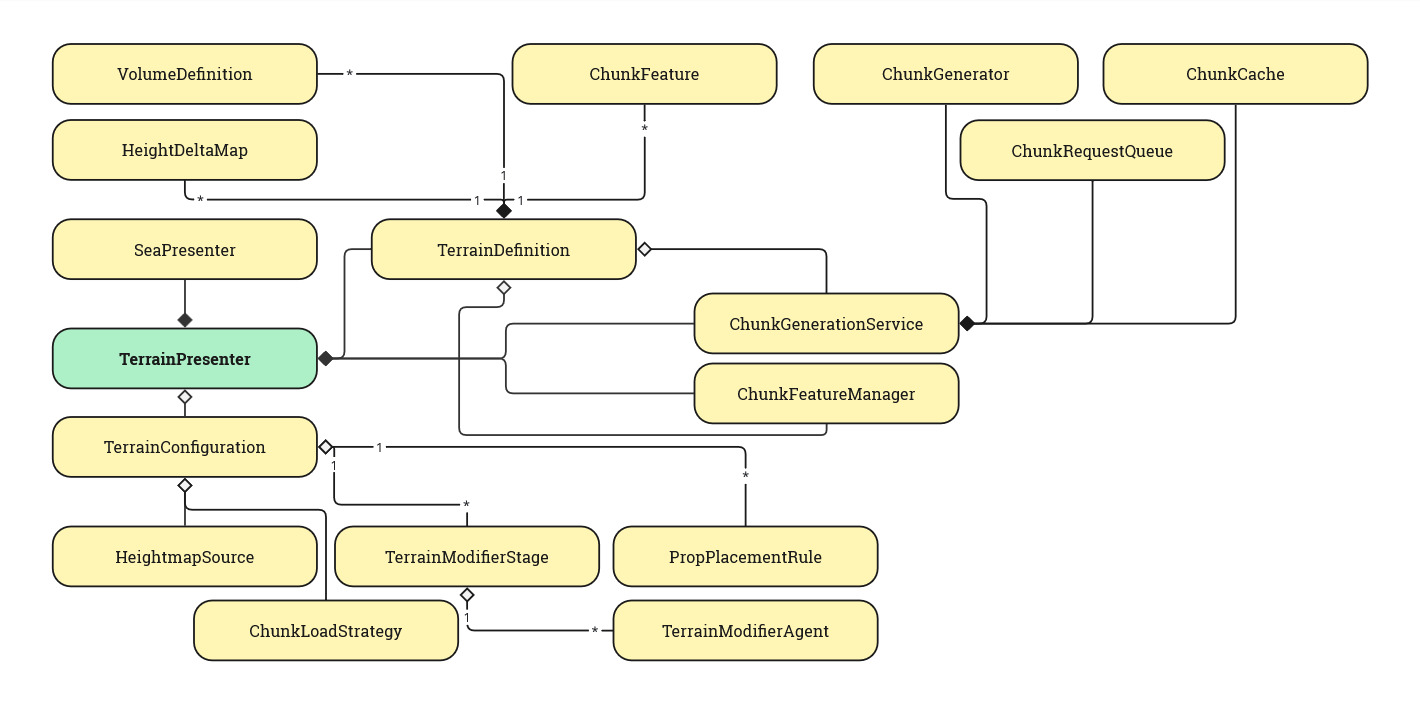
\includegraphics[width=1\textwidth]{Memoria/images/UML-TFG-Simple.jpg}
    \caption{Simplified, high-level UML class diagram for the project.}
    \label{fig:simple_uml}
\end{figure}
%% ===================================================


\section{Heightmap Generation}
This phase is the core of the entire generation system, as all subsequent stages build upon its output.
A heightmap is a discrete 2D grid of values representing heights, which are then used to generate three-dimensional terrain. % buscar cita para definición
The system implemented is very modular and aims to be designer-friendly and customizable.
The Strategy design pattern \cite{Gamma:1995:DPE} was used to achieve this, defining a generic \href{{https://github.com/fsande/TFG---Eric-Rios/blob/main/Godot-TerrainGeneration/terrain_generation/heightmap/sources/heightmap_source.gd}}{\texttt{HeightmapSource}}\footnote{\href{{https://github.com/fsande/TFG---Eric-Rios/blob/main/Godot-TerrainGeneration/terrain_generation/heightmap/sources/heightmap_source.gd}}{\textit{Godot-TerrainGeneration/terrain\_generation/heightmap/sources/heightmap\_source.gd}}} interface, including a \texttt{generate()} method, which returns an \texttt{Image}\footnote{\href{https://docs.godotengine.org/en/4.x/classes/class_image.html}{Godot \texttt{Image} Documentation} -\url{https://tinyurl.com/class-image}} object; implemented by several strategies.

As GDScript does not provide proper Interfaces or multiple inheritance, all of these objects will inherit from \texttt{HeightmapSource}, which is a subclass of Godot's \texttt{Resource}\footnote{\href{https://docs.godotengine.org/en/stable/classes/class_resource.html}{Godot \texttt{Resource} Documentation} - \url{https://tinyurl.com/resource-class}}.
This class allows for serialization of member variables and the storing of configurations, allowing users to interact with the system using the engine's default UI (see Figure \ref{fig:resource_ui_example}), without increasing code complexity.

All elements of the implementation make use of the \texttt{@tool}\footnote{\href{https://docs.godotengine.org/en/stable/tutorials/plugins/running_code_in_the_editor.html}{Running code in editor Documentation - \url{https://tinyurl.com/code-in-editor}}} annotation to run in editor time, allowing for real-time preview of generation results directly within the Godot editor, without requiring the game to be running.
%% ===================================================
\begin{figure}[H]
    \centering
    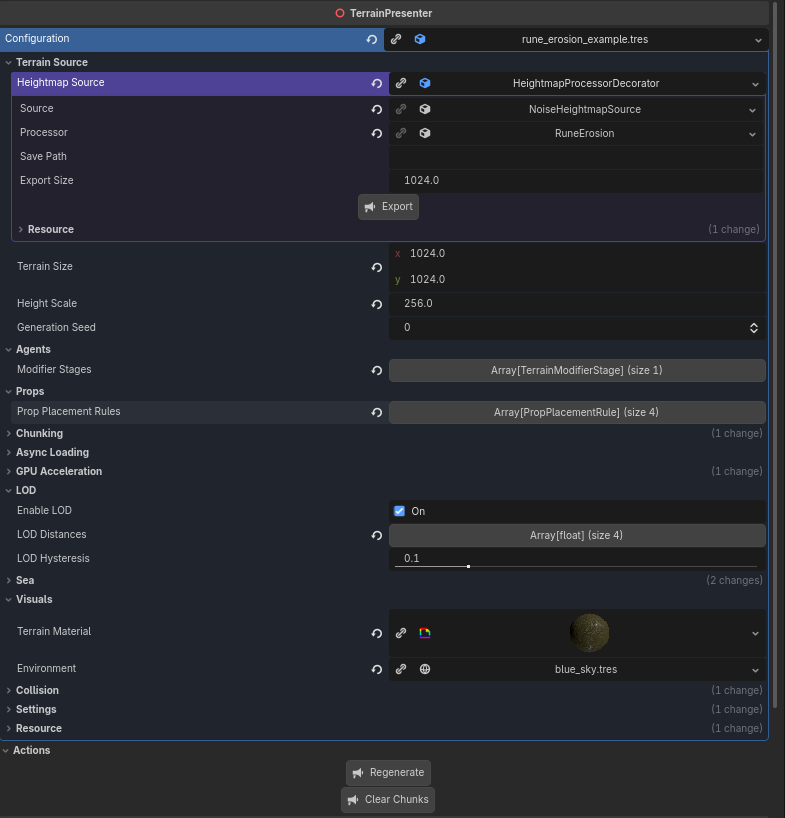
\includegraphics[width=1\textwidth]{Memoria/images/example_config_desplegado.png}
    \caption{Example configuration applied to \href{{https://github.com/fsande/TFG---Eric-Rios/blob/main/Godot-TerrainGeneration/terrain_generation/core/terrain_presenter.gd}}{\texttt{TerrainPresenter}}.}
    \label{fig:resource_ui_example}
\end{figure}
%% ===================================================
% Incluir listing aquí que explique estructura de herencia de sources

\subsection[\texttt{ImageHeightmapSource} and \texttt{TextureHeightmapSource}]{%
  \href{https://github.com/fsande/TFG---Eric-Rios/blob/main/Godot-TerrainGeneration/terrain_generation/heightmap/sources/image_heightmap_source.gd}{\texttt{ImageHeightmapSource}}\protect\footnotemark{}
  and
  \href{https://github.com/fsande/TFG---Eric-Rios/blob/main/Godot-TerrainGeneration/terrain_generation/heightmap/sources/texture_heightmap_source.gd}{\texttt{TextureHeightmapSource}}\protect\footnotemark{}}
\addtocounter{footnote}{-1}
\footnotetext{\href{https://github.com/fsande/TFG---Eric-Rios/blob/main/Godot-TerrainGeneration/terrain_generation/heightmap/sources/image_heightmap_source.gd}{\textit{Godot-TerrainGeneration/terrain\_generation/heightmap/sources/image\_heightmap\_source.gd}}}
\addtocounter{footnote}{1}
\footnotetext{\href{https://github.com/fsande/TFG---Eric-Rios/blob/main/Godot-TerrainGeneration/terrain_generation/heightmap/sources/texture_heightmap_source.gd}{\textit{Godot-TerrainGeneration/terrain\_generation/heightmap/sources/texture\_heightmap\_source.gd}}}

Both of these wrap an \texttt{Image} or \texttt{Texture2D} object respectively in the \href{{https://github.com/fsande/TFG---Eric-Rios/blob/main/Godot-TerrainGeneration/terrain_generation/heightmap/sources/heightmap_source.gd}}{\texttt{HeightmapSource}} interface.
Especially useful to import an already existing heightmap, as exemplified in Figure \ref{fig:texture_heightmap_source}.

The inheritance structure for each upcoming \href{{https://github.com/fsande/TFG---Eric-Rios/blob/main/Godot-TerrainGeneration/terrain_generation/heightmap/sources/heightmap_source.gd}}{\texttt{HeightmapSource}} subclass follows the same pattern as the one exemplified in Listing \ref{listing:image_heightmap_source}.
To avoid occupying too much space, code listings will not be used further down the document.
To access original source, follow the provided URLs.

\lstinputlisting[
    style=gdstyle,
    caption={\texttt{HeightmapSource} inheritance example. 
    \href{https://github.com/fsande/TFG---Eric-Rios/blob/main/Godot-TerrainGeneration/terrain_generation/heightmap/sources/image_heightmap_source.gd}
    {\textit{Original source}}.},
    label={listing:image_heightmap_source}
]{listings/image_heightmap_source.gd}

%% ===================================================
\begin{figure}[H]
    \centering
    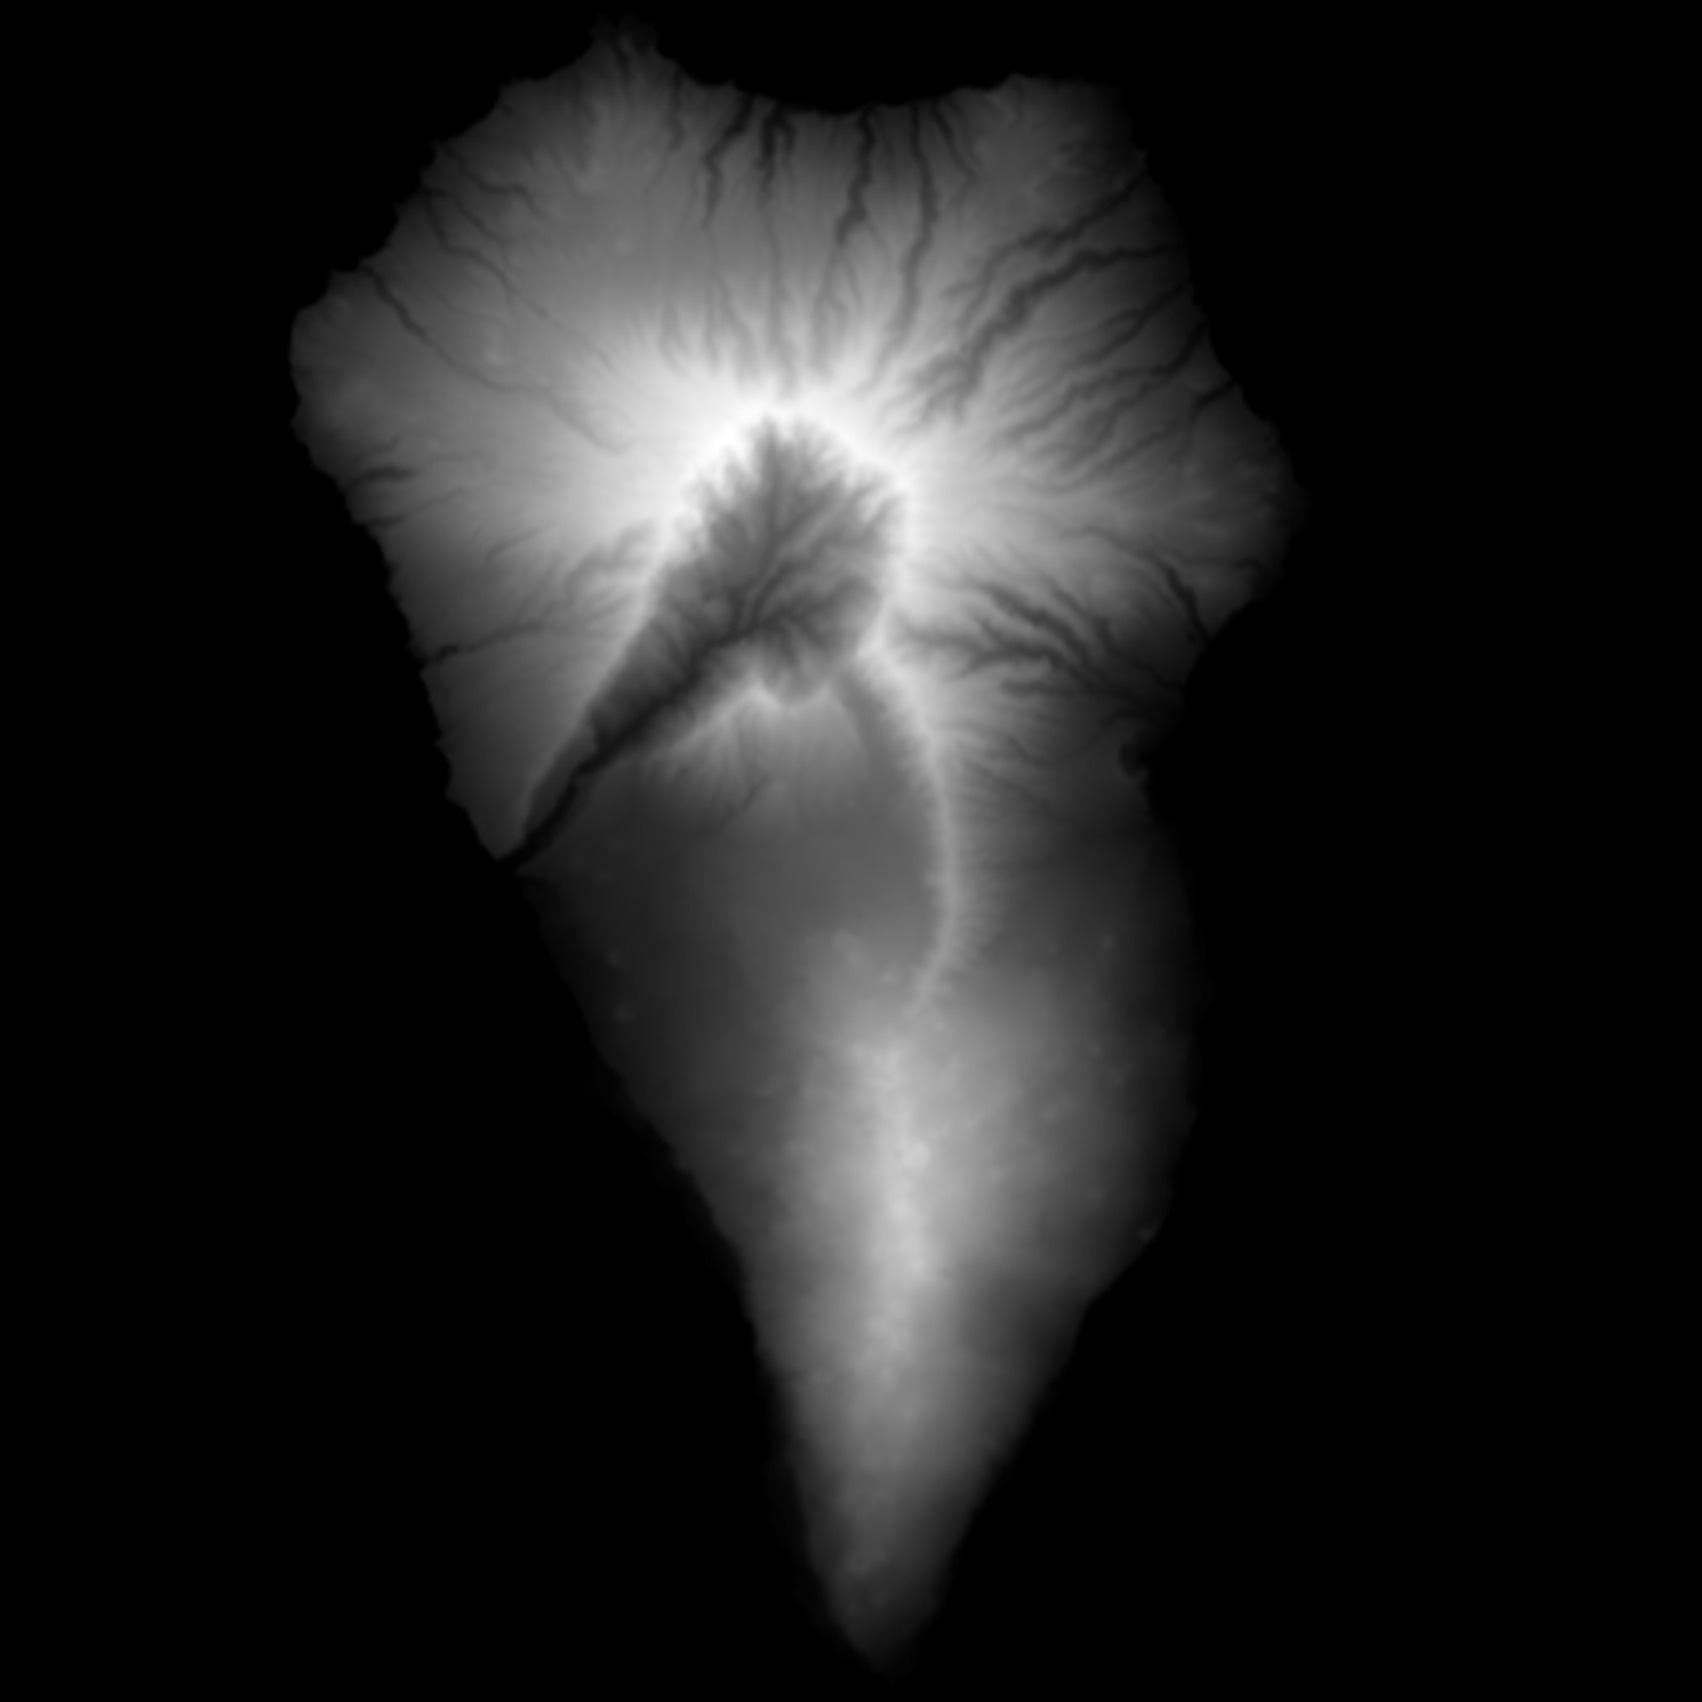
\includegraphics[width=0.49\textwidth]{Memoria/images/ultrapalma.png}
    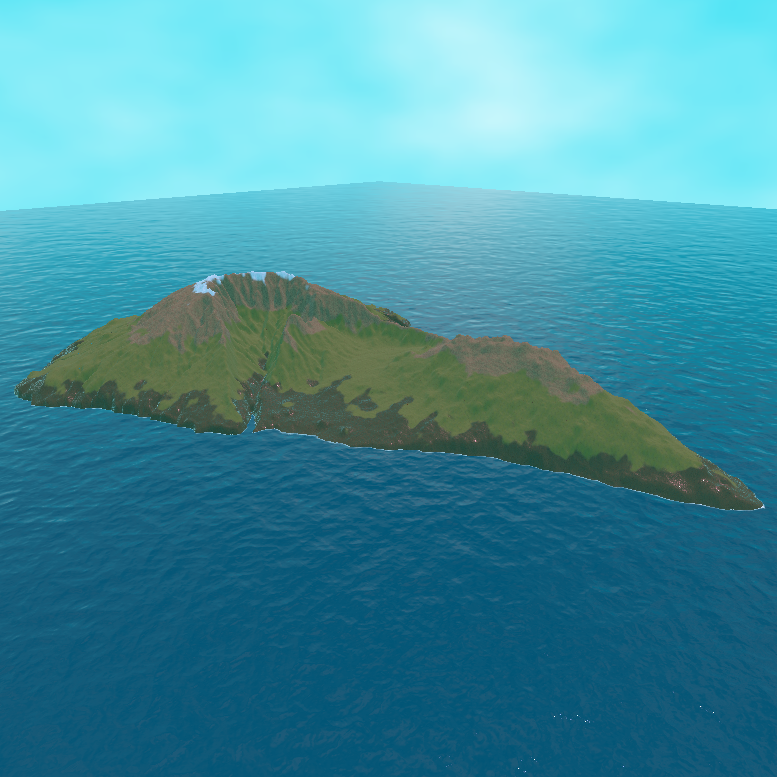
\includegraphics[width=0.49\textwidth]{Memoria/images/la_palma_3d.png}
    \caption{La Palma (Canary Islands) heightmap sourced from \url{https://tangrams.github.io/heightmapper} and its 3D representation.}
    \label{fig:texture_heightmap_source}
\end{figure}
%% ===================================================


\subsection[\texttt{NoiseHeightmapSource}]{\href{{https://github.com/fsande/TFG---Eric-Rios/blob/main/Godot-TerrainGeneration/terrain_generation/heightmap/sources/noise_heightmap_source.gd}}{\texttt{NoiseHeightmapSource}}\footnote{\href{{https://github.com/fsande/TFG---Eric-Rios/blob/main/Godot-TerrainGeneration/terrain_generation/heightmap/sources/noise_heightmap_source.gd}}{\textit{Godot-TerrainGeneration/terrain\_generation/heightmap/sources/noise\_heightmap\_source.gd}}}}
It wraps an instance of the \texttt{FastNoiseLite}\footnote{\href{https://docs.godotengine.org/en/stable/classes/class_fastnoiselite.html}{\texttt{FastNoiseLite} Godot Documentation}\\ \hspace*{1.9em}\url{https://docs.godotengine.org/en/stable/classes/class_fastnoiselite.html}} class, which provides access to the FastNoiseLite library\footnote{\href{https://github.com/Auburn/FastNoiseLite}{FastNoiseLite Library} - \url{https://github.com/Auburn/FastNoiseLite}}, a collection of various noise algorithms: \textit{Simplex}, \textit{Simplex Smooth}, \textit{Cellular}, \textit{Perlin}, \textit{Value Cubic} and \textit{Value}.
As well as providing these varied noise algorithms, it also allows extensive parametrization of the fractal, providing options for the type (\textit{FBM}, \textit{Ridged}, \textit{Ping-Pong} or \textit{None}) as well as changes to octaves, lacunarity, gain and weighted strength.
This is particularly useful, as it provides a good starting point for the generation of elevation and also aligns with this TFG's goal of customizability.
Terrain generated with \texttt{SimplexSmooth} noise is presented in Figure \ref{fig:simplex_smooth}

%% ===================================================
\begin{figure}[H]
    \centering
    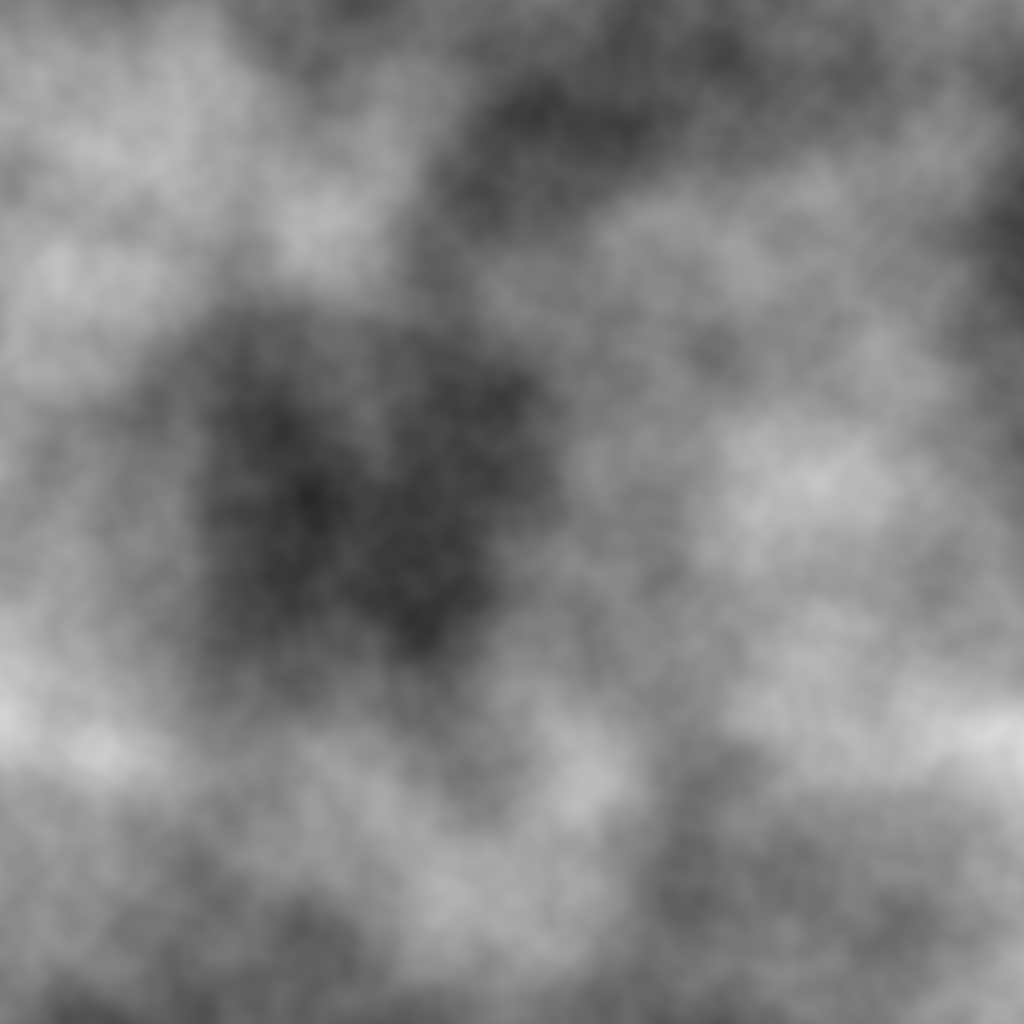
\includegraphics[width=0.49\textwidth]{Memoria/images/simplex_smooth.png}
    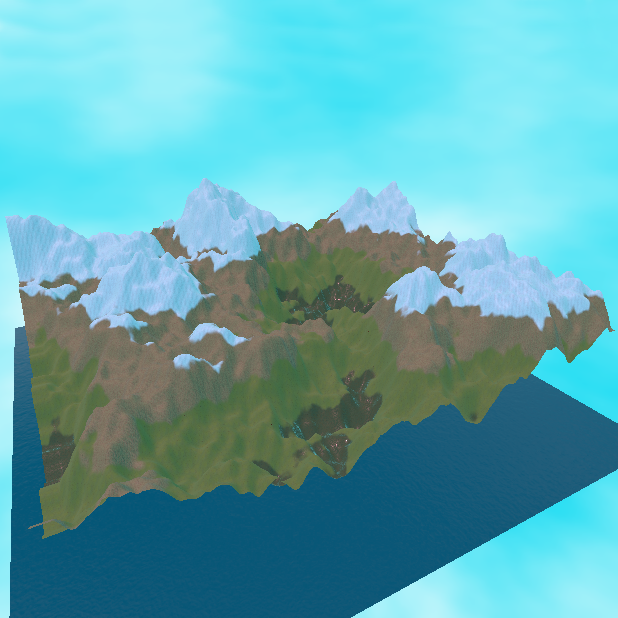
\includegraphics[width=0.49\textwidth]{Memoria/images/rendered_simplex_smooth.png}
    \caption{Heightmap generated by \textit{SimplexSmooth} noise algorithm with 5 octaves of FBM and its 3D representation.}
    \label{fig:simplex_smooth}
\end{figure}
%% ===================================================

\subsection[\texttt{HeightmapProcessorDecorator}]{\href{{https://github.com/fsande/TFG---Eric-Rios/blob/main/Godot-TerrainGeneration/terrain_generation/heightmap/sources/heightmap_processor_decorator.gd}}{\texttt{HeightmapProcessorDecorator}}\footnote{\href{{https://github.com/fsande/TFG---Eric-Rios/blob/main/Godot-TerrainGeneration/terrain_generation/heightmap/sources/heightmap_processor_decorator.gd}}{\textit{Godot-TerrainGeneration/terrain\_generation/heightmap/sources/heightmap\_processor\_decorator.gd}}}}

This class implements the \href{{https://github.com/fsande/TFG---Eric-Rios/blob/main/Godot-TerrainGeneration/terrain_generation/heightmap/sources/heightmap_source.gd}}{\texttt{HeightmapSource}} interface and makes use of the Decorator design pattern \cite{Gamma:1995:DPE} to allow different operations on a provided heightmap into the pipeline.
All processors available to this class implement the \href{{https://github.com/fsande/TFG---Eric-Rios/blob/main/Godot-TerrainGeneration/terrain_generation/heightmap/processors/heightmap_processor.gd}}{\texttt{HeightmapProcessor}}\footnote{\href{{https://github.com/fsande/TFG---Eric-Rios/blob/main/Godot-TerrainGeneration/terrain_generation/heightmap/processors/heightmap_processor.gd}}{\textit{Godot-TerrainGeneration/terrain\_generation/heightmap/processors/heightmap\_processor.gd}}} interface.

\subsubsection[\texttt{BlurProcessor}]{\href{{https://github.com/fsande/TFG---Eric-Rios/blob/main/Godot-TerrainGeneration/terrain_generation/heightmap/processors/blur_processor.gd}}{\texttt{BlurProcessor}}\footnote{\href{{https://github.com/fsande/TFG---Eric-Rios/blob/main/Godot-TerrainGeneration/terrain_generation/heightmap/processors/blur_processor.gd}}{\textit{Godot-TerrainGeneration/terrain\_generation/heightmap/processors/blur\_processor.gd}}}}

This processor implements a simple two-pass separable gaussian blur.
It provides a CPU and GPU implementation, which are equivalent.
The user can customize the blur's radius and sigma value for the Gaussian.
Edge handling is done via clamping, ensuring that sampling stays within image bounds. 
The radius is converted to an integer and defines the size of the sampling window.
While the CPU and GPU versions produce the same results, the GPU implementation is significantly more efficient, as it parallelizes the per-pixel computations (see Chapter \ref{chap:Evaluation}).
A noisy heightmap and the result of blurring it are displayed in Figure \ref{fig:blur_processor}.

%% ===================================================
\begin{figure}[H]
    \centering
    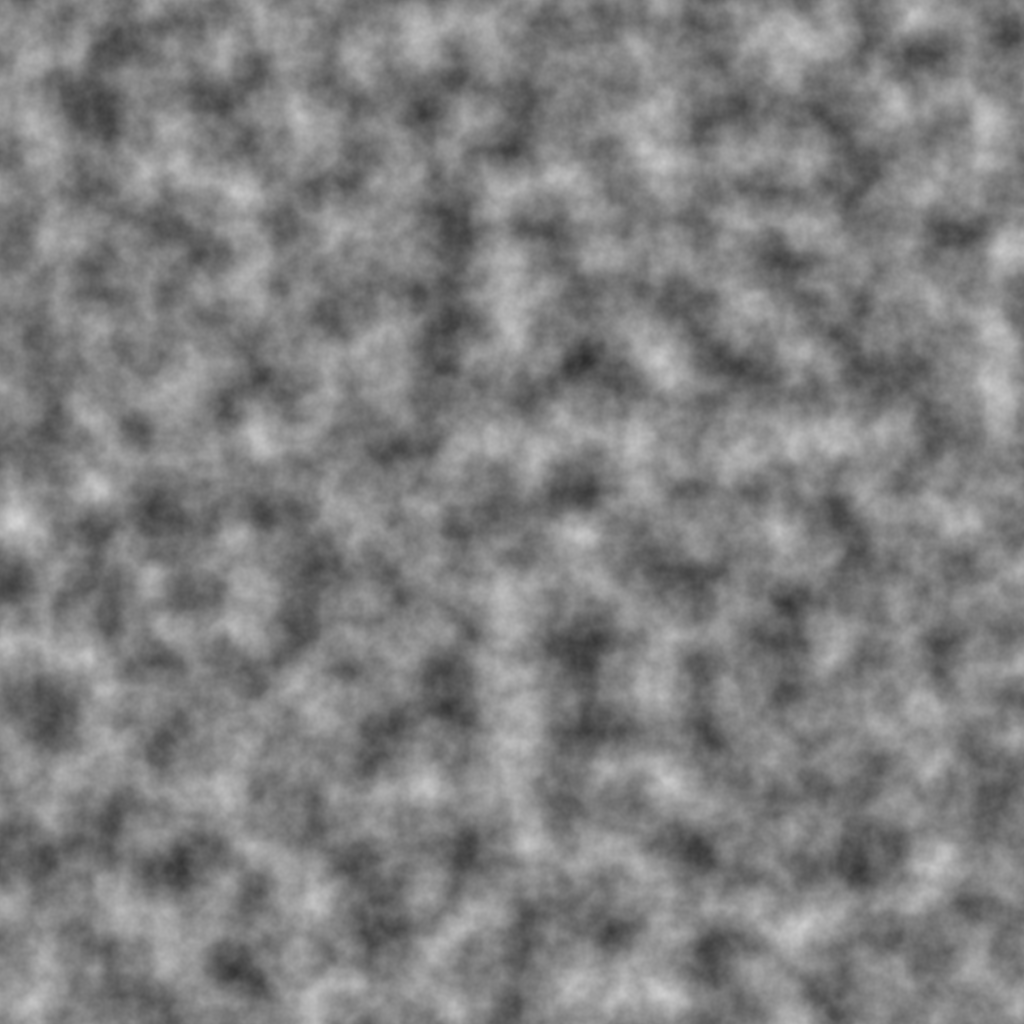
\includegraphics[width=0.325\textwidth]{Memoria/images/pre_blur_noise.png}
    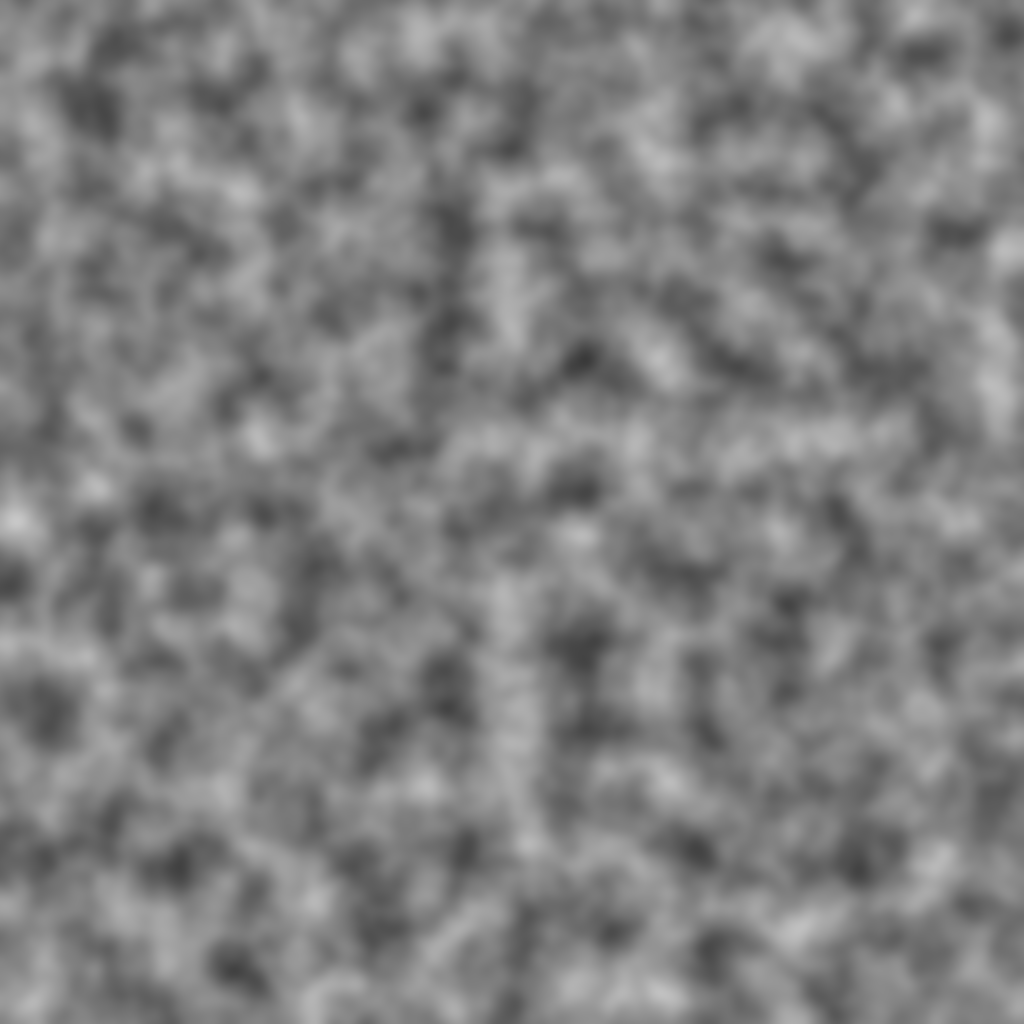
\includegraphics[width=0.325\textwidth]{Memoria/images/post_blur_noise.png}
    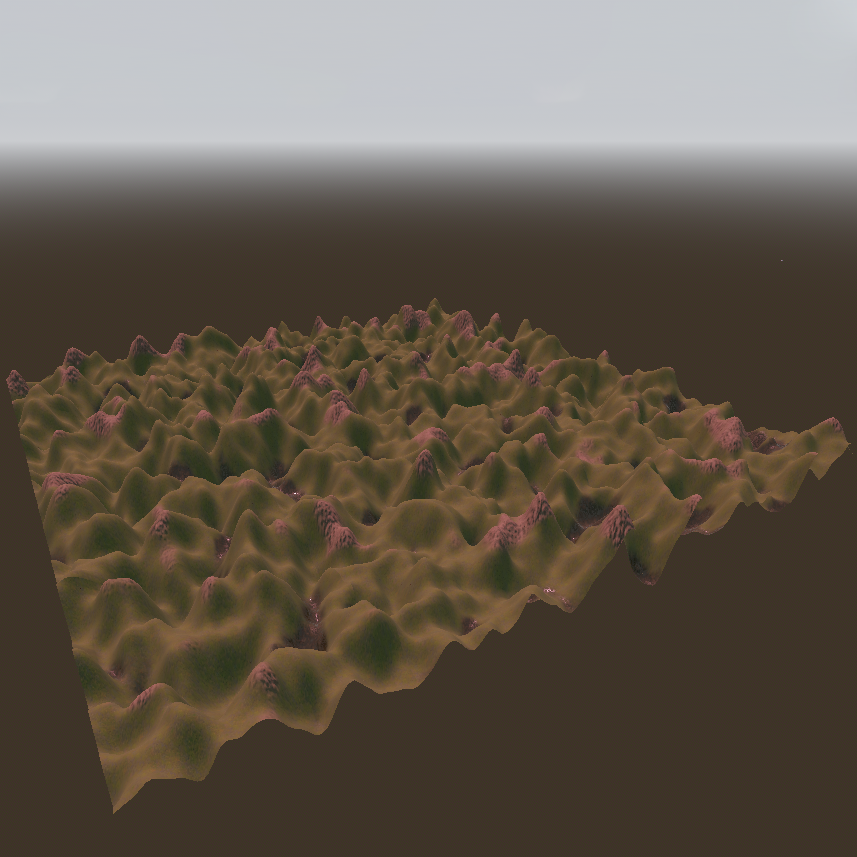
\includegraphics[width=0.325\textwidth]{Memoria/images/rendered_blur_terrain.png}
    \caption{Base heightmap, the result of blurring it with a radius of 15 pixels and its 3D rendering.}
    \label{fig:blur_processor}
\end{figure}
%% ===================================================

\subsubsection[\texttt{MaskProcessor}]{\href{{https://github.com/fsande/TFG---Eric-Rios/blob/main/Godot-TerrainGeneration/terrain_generation/heightmap/processors/mask_processor.gd}}{\texttt{MaskProcessor}}\footnote{\href{{https://github.com/fsande/TFG---Eric-Rios/blob/main/Godot-TerrainGeneration/terrain_generation/heightmap/processors/mask_processor.gd}}{\textit{Godot-TerrainGeneration/terrain\_generation/heightmap/processors/mask\_processor.gd}}}}
This processor takes a mask image and a \href{{https://github.com/fsande/TFG---Eric-Rios/blob/main/Godot-TerrainGeneration/terrain_generation/heightmap/sources/heightmap_source.gd}}{\texttt{HeightmapSource}}.
The areas of the mask image that are white will keep the source height, while the ones that are black will nullify any height. 
This allows a designer to provide a silhouette of the terrain they want to generate and let the application perform the rest of height generation.
Optionally, transitions can be defined between the white and black part of the images, to provide a less abrupt transition from terrain to sea.
Another option to reduce the abruptness of the transitions makes use of the \href{{https://github.com/fsande/TFG---Eric-Rios/blob/main/Godot-TerrainGeneration/terrain_generation/heightmap/processors/blur_processor.gd}}{\texttt{BlurProcessor}}, blurring the borders of the mask image.
There are two implemented transitions: \href{https://github.com/fsande/TFG---Eric-Rios/blob/main/Godot-TerrainGeneration/terrain_generation/heightmap/transitions/beach_transition.gd}{\texttt{BeachTransition}}\footnote{\href{https://github.com/fsande/TFG---Eric-Rios/blob/main/Godot-TerrainGeneration/terrain_generation/heightmap/transitions/beach_transition.gd}{Godot-TerrainGeneration/terrain\_generation/heightmap/transitions/beach\_transition.gd}} and \href{https://github.com/fsande/TFG---Eric-Rios/blob/main/Godot-TerrainGeneration/terrain_generation/heightmap/transitions/cliff_transition.gd}{\texttt{CliffTransition}}\footnote{\href{https://github.com/fsande/TFG---Eric-Rios/blob/main/Godot-TerrainGeneration/terrain_generation/heightmap/transitions/cliff_transition.gd}{Godot-TerrainGeneration/terrain\_generation/heightmap/transitions/cliff\_transition.gd}}, which provide variation, although, thanks to the Strategy pattern also implemented here, the system can be easily extended.
This is currently only implemented on the CPU.
An example using Keep It Clean's \cite{Cruz:2025:PBC, Herrera:2025:PBC} logo as a mask (with the developers' permissions) is pictured in Figure \ref{fig:mask_processor}

%% ===================================================
\begin{figure}[H]
    \centering
    
\includegraphics[width=0.41\textwidth]{Memoria/images/keep_it_clean_logo.png}
    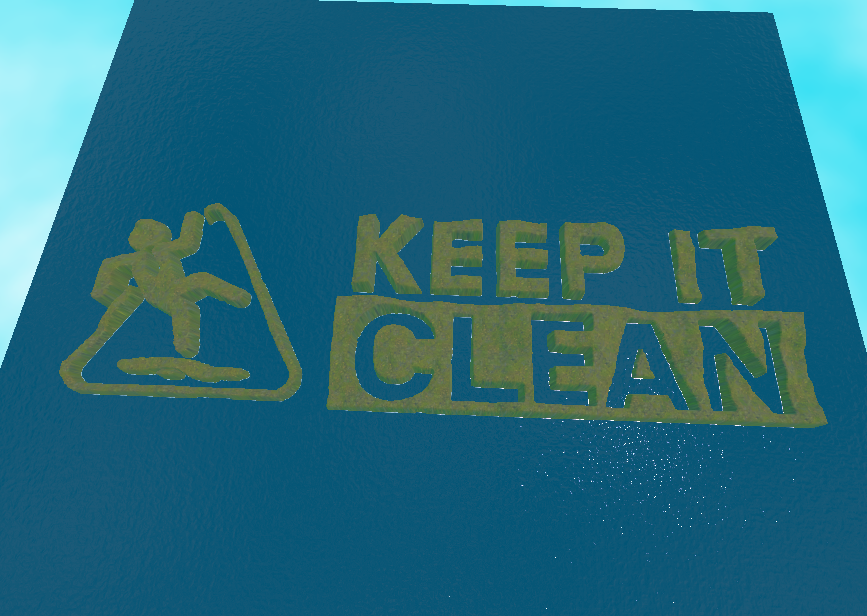
\includegraphics[width=0.58\textwidth]{Memoria/images/rendered_mask_agent.png}
    \caption{Mask applied on top of basic \textit{Simplex} noise.}
    \label{fig:mask_processor}
\end{figure}
%% ===================================================

\subsubsection[\texttt{ContrastProcessor}]{\href{https://github.com/fsande/TFG---Eric-Rios/blob/main/Godot-TerrainGeneration/terrain_generation/heightmap/processors/contrast_processor.gd}{\texttt{ContrastProcessor}}\footnote{\href{https://github.com/fsande/TFG---Eric-Rios/blob/main/Godot-TerrainGeneration/terrain_generation/heightmap/processors/contrast_processor.gd}{\textit{Godot-TerrainGeneration/terrain\_generation/heightmap/processors/contrast\_processor.gd}}}}

This processor analyses the minimum and maximum values in the provided heightmap and remaps all values to fit within the target range with user-defined percentiles to map the maximum and minimum to.
This is useful to ensure that heightmaps use the full dynamic range or to constrain values to specific bounds.
It is implemented in both GPU and CPU.
An example of usage on a low-contrast base heightmap is shown in Figure \ref{fig:contrast_processor}.

%% ===================================================
\begin{figure}[H]
    \centering
    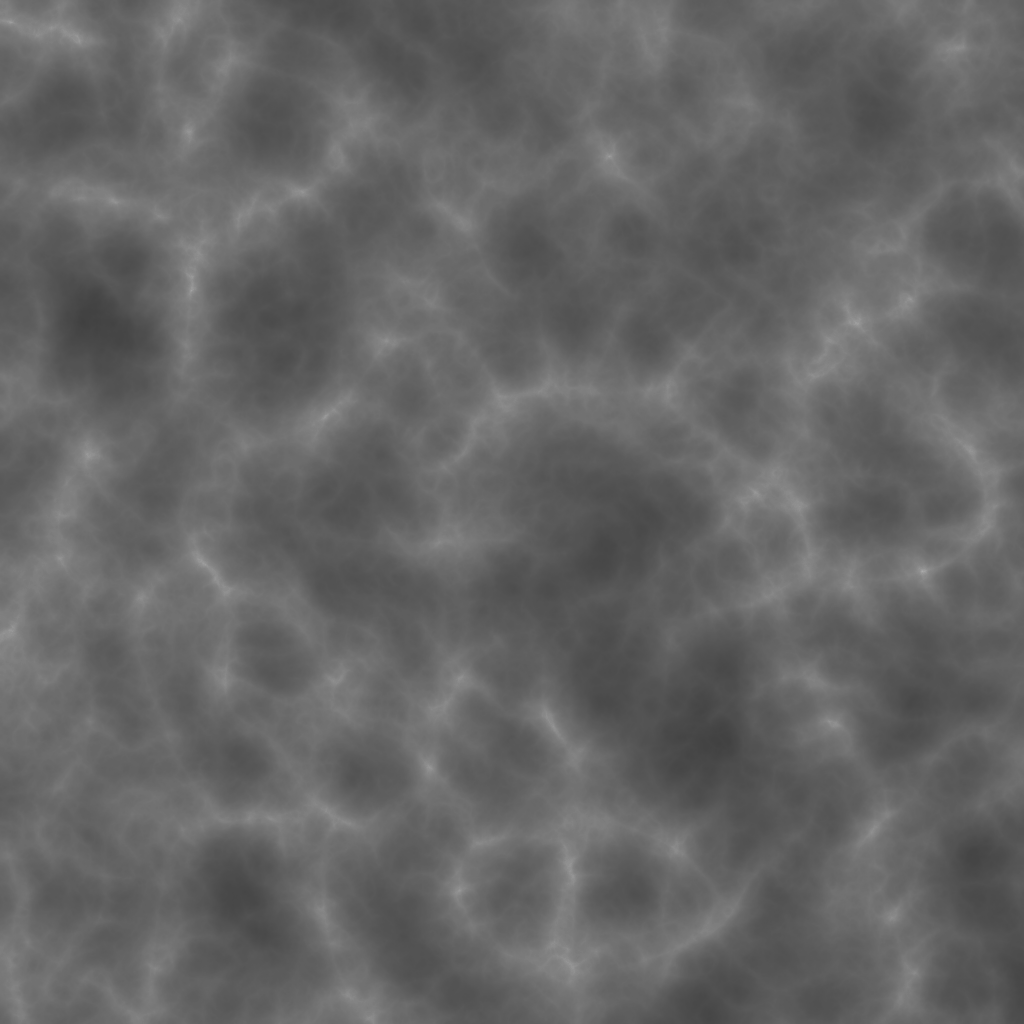
\includegraphics[width=0.49\textwidth]{Memoria/images/ridged_noise_low_contrast.png}
    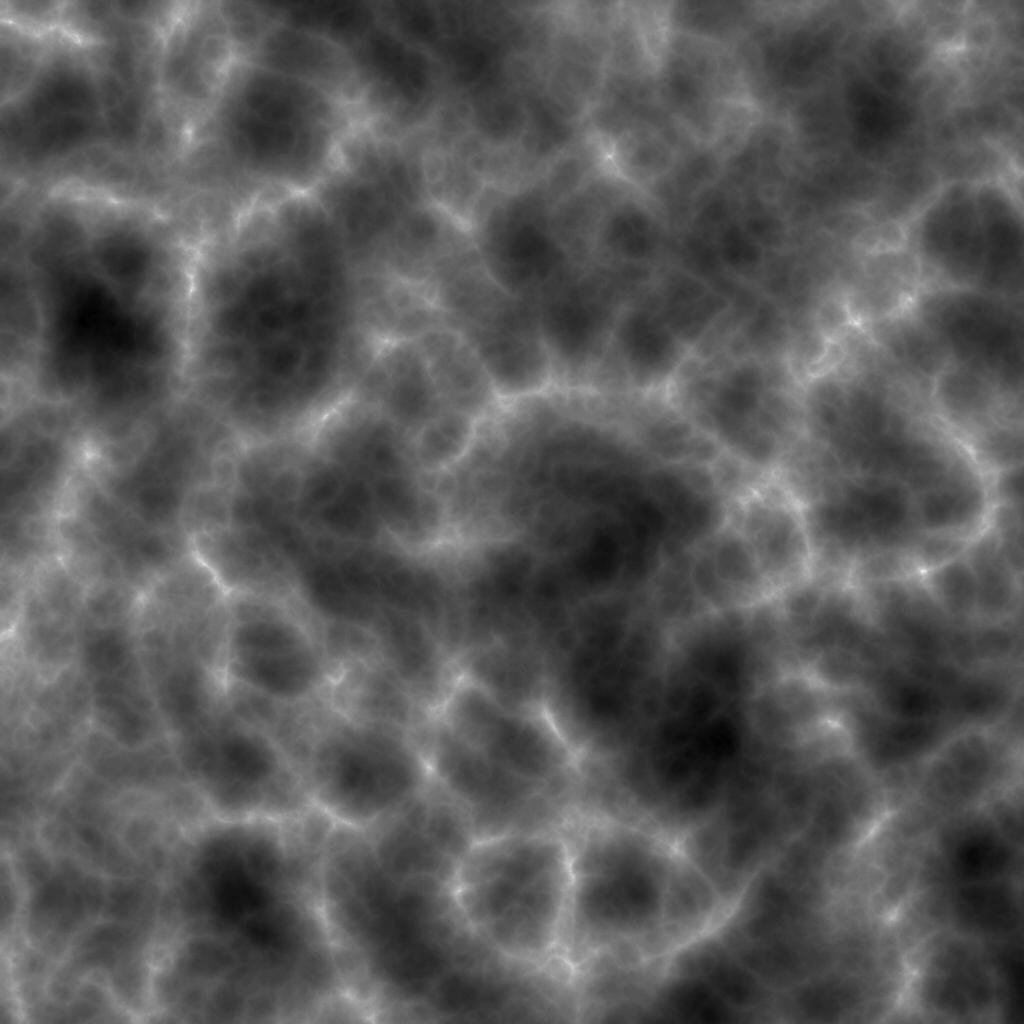
\includegraphics[width=0.49\textwidth]{Memoria/images/ridged_norm.png}
    \caption{Low-contrast noise before and after normalization.}
    \label{fig:contrast_processor}
\end{figure}
%% ===================================================

\subsubsection[\texttt{ThermalErosionProcessor}]{\href{https://github.com/fsande/TFG---Eric-Rios/blob/main/Godot-TerrainGeneration/terrain_generation/heightmap/processors/thermal_erosion_processor.gd}{\texttt{ThermalErosionProcessor}}\footnote{\href{https://github.com/fsande/TFG---Eric-Rios/blob/main/Godot-TerrainGeneration/terrain_generation/heightmap/processors/thermal_erosion_processor.gd}{\textit{Godot-TerrainGeneration/terrain\_generation/heightmap/processors/thermal\_erosion\_processor.gd}}}}
This class implements an adaptation of the pseudocode for the thermal erosion proposed by Olsen \cite{Olsen:2004:RPT}.
The GPU implementation is currently not completely equivalent to the CPU version, as the CPU algorithm distributes eroded material proportionally to neighbouring height differences, while the GPU implementation uses a simplified gather-based redistribution model optimized for parallel execution.
This approximation avoids costly atomic operations and synchronization issues on the GPU.
The results are good, as seen in Figure \ref{fig:thermal_processor}.

%% ===================================================
\begin{figure}[H]
    \centering
    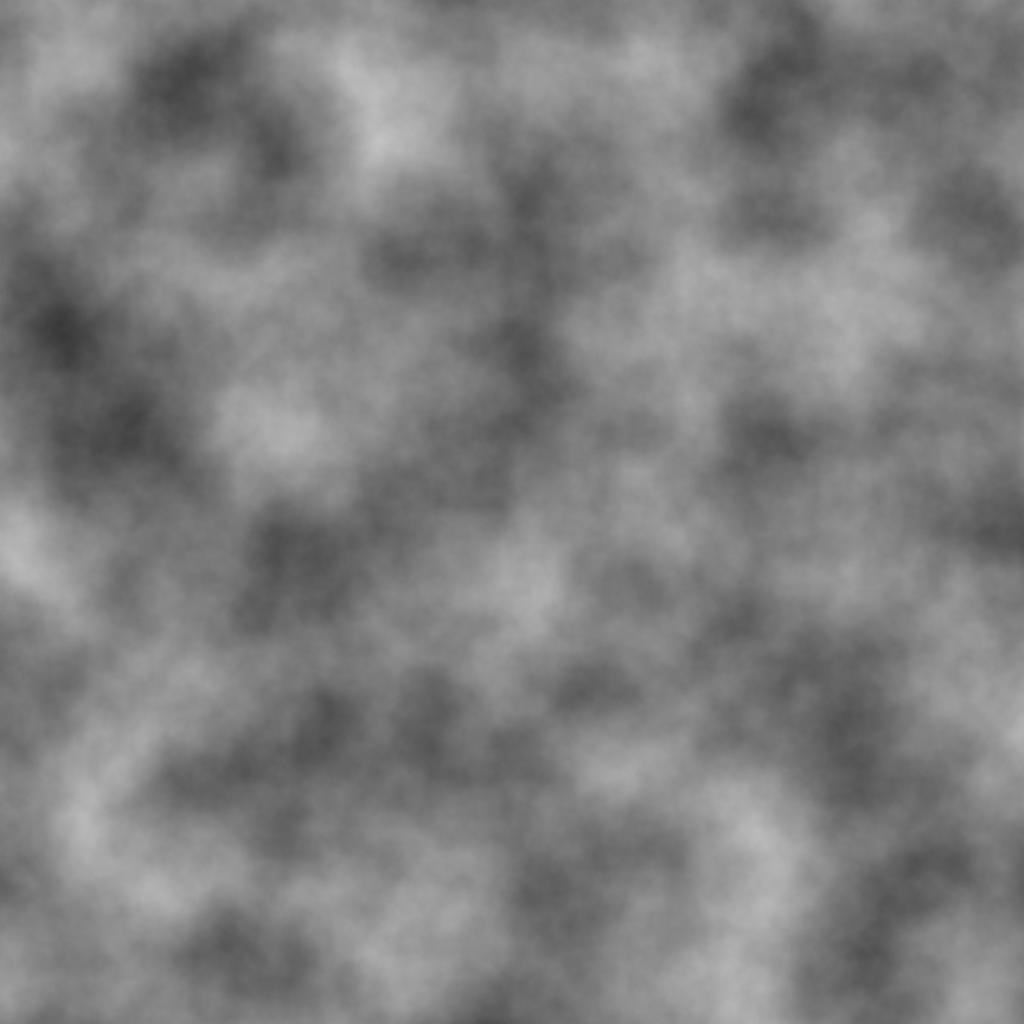
\includegraphics[width=0.325\textwidth]{Memoria/images/before_thermal_erosion.png}
    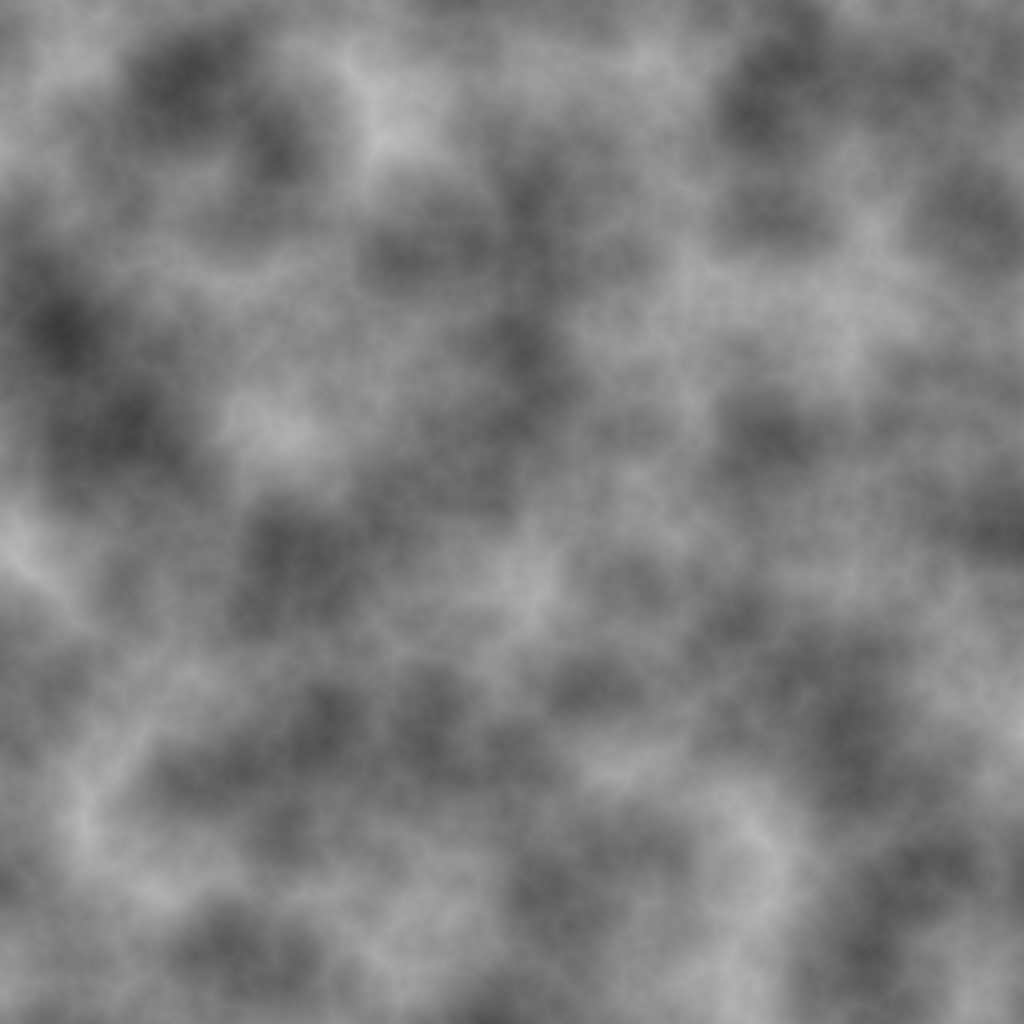
\includegraphics[width=0.325\textwidth]{Memoria/images/thermal_eroded.png}
    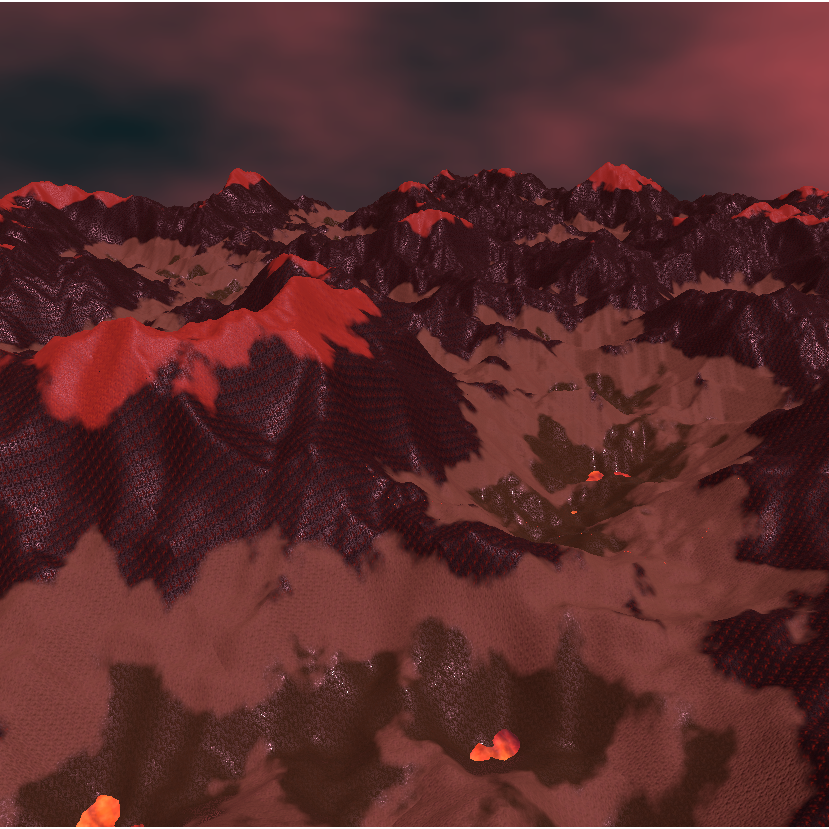
\includegraphics[width=0.325\textwidth]{Memoria/images/rendered_thermal.png}
    \caption{Base heightmap, the result of applying thermal erosion and its 3D rendering.}
    \label{fig:thermal_processor}
\end{figure}
%% ===================================================


\subsubsection[\texttt{RuneErosion}]{\href{https://github.com/fsande/TFG---Eric-Rios/blob/main/Godot-TerrainGeneration/terrain_generation/heightmap/processors/rune_erosion.gd}{\texttt{RuneErosion}}\footnote{\href{https://github.com/fsande/TFG---Eric-Rios/blob/main/Godot-TerrainGeneration/terrain_generation/heightmap/processors/rune_erosion.gd}{\textit{Godot-TerrainGeneration/terrain\_generation/heightmap/processors/rune\_erosion.gd}}}}

This class wraps a compute shader implementing a version of the \textit{Fast and Gorgeous Erosion Filter} designed by Rune Skovbo Johansen\footnote{\href{https://blog.runevision.com/2026/03/fast-and-gorgeous-erosion-filter.html}{Blog detailing erosion filter implementation}\\ \hspace*{1.9em}\url{https://blog.runevision.com/2026/03/fast-and-gorgeous-erosion-filter.html}}.
The implementation differs mainly in input and output, as the requirements in the implemented PCG system differ from those in Shadertoy\footnote{\href{https://www.shadertoy.com/}{Shadertoy site} - \url{https://www.shadertoy.com/}}.

This filter works best when applied onto a low-frequency noise base heightmap, as exemplified in Figure \ref{fig:rune_erosion}.

%% ===================================================
\begin{figure}[H]
    \centering
    
\includegraphics[width=0.325\textwidth]{Memoria/images/noise_pre_rune.png}
    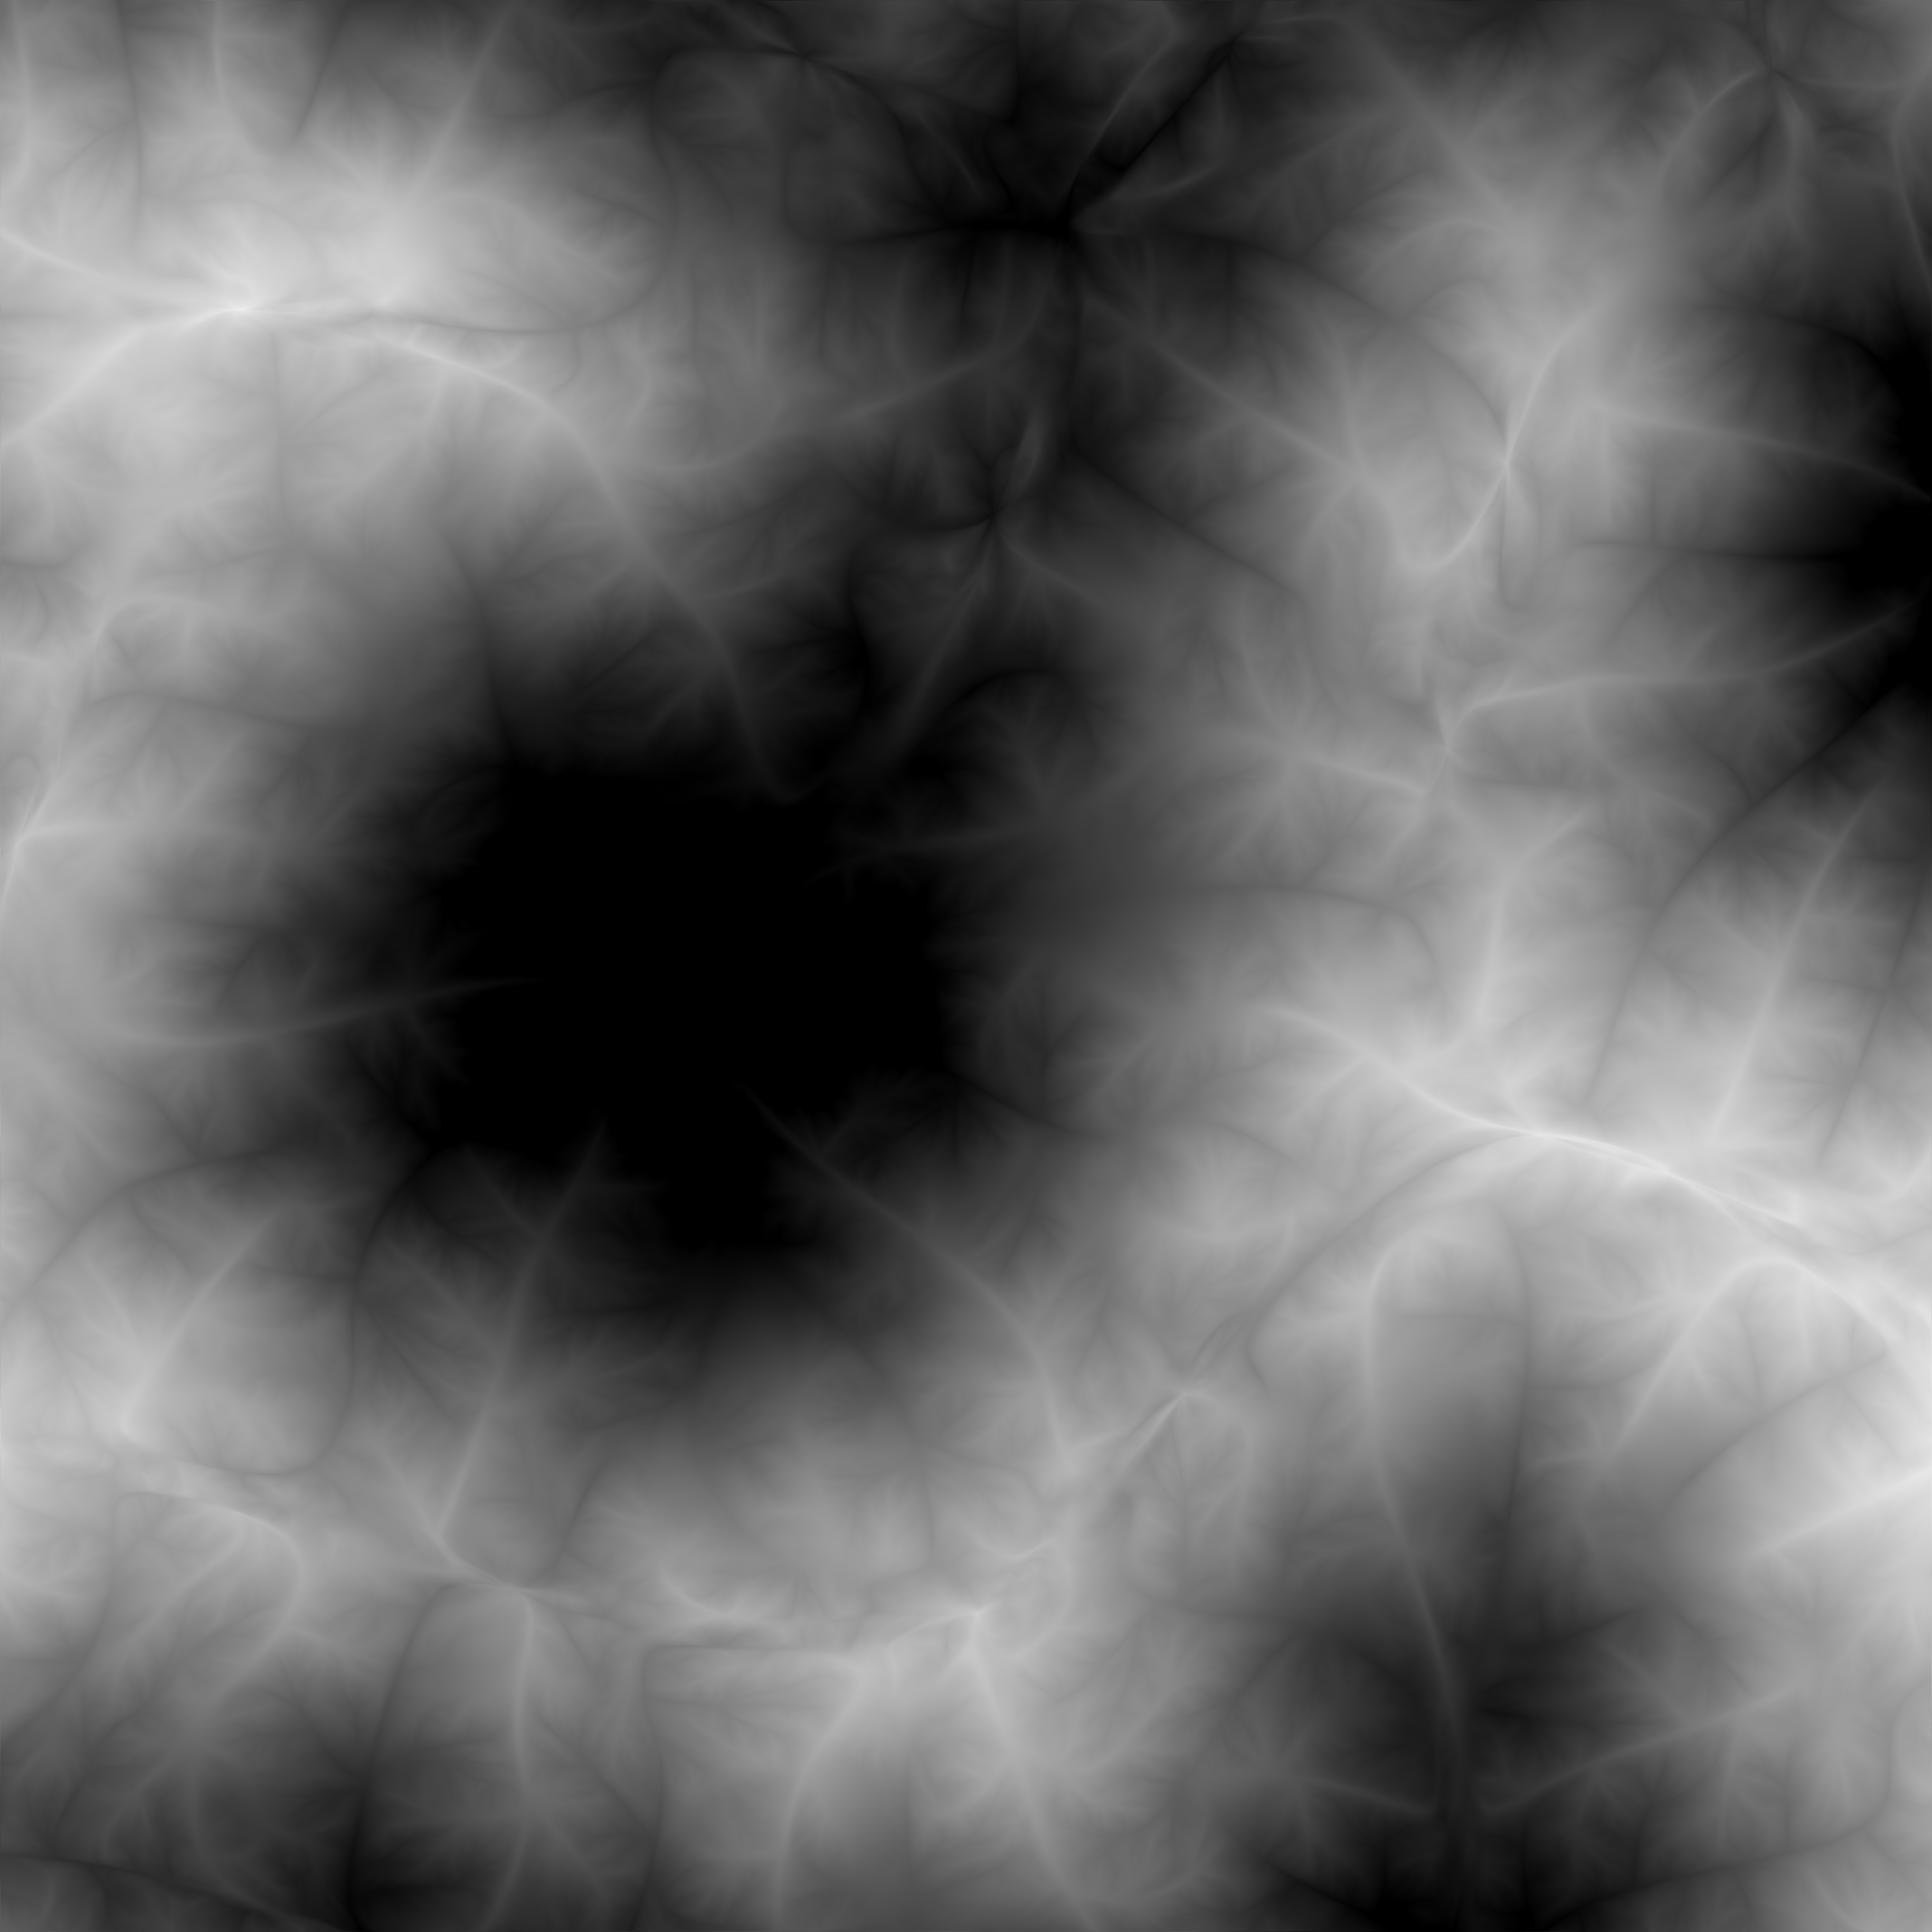
\includegraphics[width=0.325\textwidth]{Memoria/images/rune_eroded.png}
    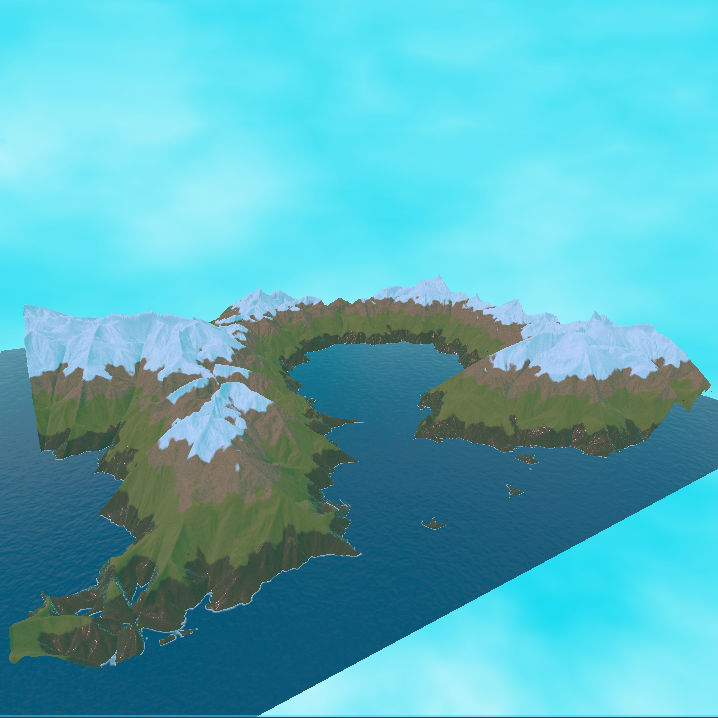
\includegraphics[width=0.325\textwidth]{Memoria/images/rendered_rune.png}
    \caption{Heightmap generated by applying \href{https://github.com/fsande/TFG---Eric-Rios/blob/main/Godot-TerrainGeneration/terrain_generation/heightmap/processors/rune_erosion.gd}{\texttt{RuneErosion}} on top of a \texttt{SimplexSmooth}, no fractal base heightmap.}
    \label{fig:rune_erosion}
\end{figure}
%% ===================================================

\subsection[\texttt{CompositeHeightmapSource}]{\href{https://github.com/fsande/TFG---Eric-Rios/blob/main/Godot-TerrainGeneration/terrain_generation/heightmap/sources/composite_heightmap_source.gd}{\texttt{CompositeHeightmapSource}}\footnote{\href{https://github.com/fsande/TFG---Eric-Rios/blob/main/Godot-TerrainGeneration/terrain_generation/heightmap/sources/composite_heightmap_source.gd}{\textit{Godot-TerrainGeneration/terrain\_generation/heightmap/sources/composite\_heightmap\_source.gd}}}}

This class takes an arbitrary number of \href{{https://github.com/fsande/TFG---Eric-Rios/blob/main/Godot-TerrainGeneration/terrain_generation/heightmap/sources/heightmap_source.gd}}{\texttt{HeightmapSource}} objects and composites them.
The way they are mixed is defined by the chosen \href{https://github.com/fsande/TFG---Eric-Rios/blob/main/Godot-TerrainGeneration/terrain_generation/heightmap/combiners/heightmap_combiner.gd}{\texttt{HeightmapCombiner}}\footnote{\href{https://github.com/fsande/TFG---Eric-Rios/blob/main/Godot-TerrainGeneration/terrain_generation/heightmap/combiners/heightmap_combiner.gd}{\textit{Godot-TerrainGeneration/terrain\_generation/heightmap/combiners/heightmap\_combiner.gd}}}, another interface following the Strategy pattern.
When working with sources of different resolutions, the smaller ones are upscaled to match the larger ones.
The currently available \href{https://github.com/fsande/TFG---Eric-Rios/blob/main/Godot-TerrainGeneration/terrain_generation/heightmap/combiners/heightmap_combiner.gd}{\texttt{HeightmapCombiner}}s are:

\subsubsection[\texttt{AverageCombiner}]{\href{https://github.com/fsande/TFG---Eric-Rios/blob/main/Godot-TerrainGeneration/terrain_generation/heightmap/combiners/average_combiner.gd}{\texttt{AverageCombiner}}\footnote{\href{https://github.com/fsande/TFG---Eric-Rios/blob/main/Godot-TerrainGeneration/terrain_generation/heightmap/combiners/average_combiner.gd}{\textit{Godot-TerrainGeneration/terrain\_generation/heightmap/combiners/average\_combiner.gd}}}}

Takes the average for each pixel and returns it.

\subsubsection[\texttt{WeightedCombiner}]{\href{https://github.com/fsande/TFG---Eric-Rios/blob/main/Godot-TerrainGeneration/terrain_generation/heightmap/combiners/weighted_combiner.gd}{\texttt{WeightedCombiner}}\footnote{\href{https://github.com/fsande/TFG---Eric-Rios/blob/main/Godot-TerrainGeneration/terrain_generation/heightmap/combiners/weighted_combiner.gd}{\textit{Godot-TerrainGeneration/terrain\_generation/heightmap/combiners/weighted\_combiner.gd}}}}

A weight is assigned to each \href{{https://github.com/fsande/TFG---Eric-Rios/blob/main/Godot-TerrainGeneration/terrain_generation/heightmap/sources/heightmap_source.gd}}{\texttt{HeightmapSource}} provided.
They are normalized and applied in the same way the \href{https://github.com/fsande/TFG---Eric-Rios/blob/main/Godot-TerrainGeneration/terrain_generation/heightmap/combiners/average_combiner.gd}{\texttt{AverageCombiner}} does.

\subsubsection[\texttt{MultiplicationCombiner}]{\href{https://github.com/fsande/TFG---Eric-Rios/blob/main/Godot-TerrainGeneration/terrain_generation/heightmap/combiners/multiplication_combiner.gd}{\texttt{MultiplicationCombiner}}\footnote{\href{https://github.com/fsande/TFG---Eric-Rios/blob/main/Godot-TerrainGeneration/terrain_generation/heightmap/combiners/multiplication_combiner.gd}{\textit{Godot-TerrainGeneration/terrain\_generation/heightmap/combiners/multiplication\_combiner.gd}}}}

Multiplies the value of each respective pixel.
Allows for easy height variation in different areas.
Especially useful in combination with with cellular noise.

\section{Agent Modification}

The implementation of agents for terrain generation is inspired by the basis presented by Doran and Parberry \cite{Doran:2010:CPT} and follows a similar architecture to the basic heightmap generation.
Agents are organized in a pipeline, which is divided into several stages.
These can be sequential, where one agent is executed after the other; and conditional, where a given \href{https://github.com/fsande/TFG---Eric-Rios/blob/main/Godot-TerrainGeneration/terrain_generation/core/conditions/terrain_condition.gd}{\texttt{TerrainCondition}}\footnote{\href{https://github.com/fsande/TFG---Eric-Rios/blob/main/Godot-TerrainGeneration/terrain_generation/core/conditions/terrain_condition.gd}{\textit{Godot-TerrainGeneration/terrain\_generation/core/conditions/terrain\_condition.gd}}} evaluates a terrain metric, such as slope, size, etc.
An agent is chosen accordingly after evaluation.
An implementation of a parallel stage was begun, as the referenced \cite{Doran:2010:CPT} implementation relies on concurrency.
However, the difficulty of ensuring determinism while maintaining the benefits tied to parallel agent execution (the referenced paper seems to accept non-deterministic behaviour) has led to the abandonment of this avenue for the current project, as we value replicability over performance.

Agents function not by directly modifying the heightmap generated in the previous phase, but by sampling it and generating localized differences (deltas) that are used further down the pipeline.
The deltas are only taken into account during generation when a generated chunk is affected by them. 
To achieve this, each delta has an Axis-Aligned Bounding Box (\texttt{AABB}\footnote{\href{https://docs.godotengine.org/en/stable/classes/class_aabb.html}{\texttt{AABB} Godot Documentation}\\ \hspace*{1.9em}\url{https://docs.godotengine.org/en/stable/classes/class_aabb.html}}) to represent its world-space bounds.
Deltas can be either \href{https://github.com/fsande/TFG---Eric-Rios/blob/main/Godot-TerrainGeneration/terrain_generation/core/height_delta_map.gd}{\texttt{HeightDeltaMap}}\footnote{\href{https://github.com/fsande/TFG---Eric-Rios/blob/main/Godot-TerrainGeneration/terrain_generation/core/height_delta_map.gd}{\textit{Godot-TerrainGeneration/terrain\_generation/core/height\_delta\_map.gd}}} or \href{https://github.com/fsande/TFG---Eric-Rios/blob/main/Godot-TerrainGeneration/terrain_generation/agents/volume_definition.gd}{\texttt{VolumeDefinition}}\footnote{\href{https://github.com/fsande/TFG---Eric-Rios/blob/main/Godot-TerrainGeneration/terrain_generation/agents/volume_definition.gd}{\textit{Godot-TerrainGeneration/terrain\_generation/agents/volume\_definition.gd}}}.

\href{https://github.com/fsande/TFG---Eric-Rios/blob/main/Godot-TerrainGeneration/terrain_generation/core/height_delta_map.gd}{\texttt{HeightDeltaMap}} are simple textures which alter the terrain's height. 
Instances of the class have a \href{https://github.com/fsande/TFG---Eric-Rios/blob/main/Godot-TerrainGeneration/terrain_generation/core/blending/height_blend_strategy.gd}{\texttt{HeightBlendStrategy}}\footnote{\href{https://github.com/fsande/TFG---Eric-Rios/blob/main/Godot-TerrainGeneration/terrain_generation/core/blending/height_blend_strategy.gd}{\textit{Godot-TerrainGeneration/terrain\_generation/core/blending/height\_blend\_strategy.gd}}}, which defines how the generated texture affects the underlying heightmap.
\href{https://github.com/fsande/TFG---Eric-Rios/blob/main/Godot-TerrainGeneration/terrain_generation/core/blending/additive_blend_strategy.gd}{\texttt{AdditiveBlendStrategy}}, \href{https://github.com/fsande/TFG---Eric-Rios/blob/main/Godot-TerrainGeneration/terrain_generation/core/blending/max_blend_strategy.gd}{\texttt{MaxBlendStrategy}}, \href{https://github.com/fsande/TFG---Eric-Rios/blob/main/Godot-TerrainGeneration/terrain_generation/core/blending/min_blend_strategy.gd}{\texttt{MinBlendStrategy}}, \href{https://github.com/fsande/TFG---Eric-Rios/blob/main/Godot-TerrainGeneration/terrain_generation/core/blending/multiplicative_blend_strategy.gd}{\texttt{MultiplicativeBlendStrategy}}, \href{https://github.com/fsande/TFG---Eric-Rios/blob/main/Godot-TerrainGeneration/terrain_generation/core/blending/replace_blend_strategy.gd}{\texttt{ReplaceBlendStrategy}}, and \href{https://github.com/fsande/TFG---Eric-Rios/blob/main/Godot-TerrainGeneration/terrain_generation/core/blending/smooth_blend_strategy.gd}{\texttt{SmoothBlendStrategy}} have been implemented as of this point in development.

The implementation of \href{https://github.com/fsande/TFG---Eric-Rios/blob/main/Godot-TerrainGeneration/terrain_generation/agents/volume_definition.gd}{\texttt{VolumeDefinition}} is slightly more complex.
Heightmaps, being two-dimensional, are limited in what can be translated to 3D geometry.
They cannot, for example, directly be converted to terrain with overhangs or caves.
\href{https://github.com/fsande/TFG---Eric-Rios/blob/main/Godot-TerrainGeneration/terrain_generation/agents/volume_definition.gd}{\texttt{VolumeDefinition}} was implemented to provide agents with the ability of generating such three-dimensional features through the use of Constructive Solid Geometry (CSG) and other methods.

Just as the heightmap architecture, the agents make use of Godot's \texttt{Resource} class for extensive parametrization, each agent having a corresponding configuration class.
The following agents have been implemented, some of them based on the pseudocode provided in \cite{Doran:2010:CPT}:

\subsection[\texttt{TerrainRaiseAgent}]{\href{https://github.com/fsande/TFG---Eric-Rios/blob/main/Godot-TerrainGeneration/terrain_generation/agents/terrain_raise_agent.gd}{\texttt{TerrainRaiseAgent}}\footnote{\href{https://github.com/fsande/TFG---Eric-Rios/blob/main/Godot-TerrainGeneration/terrain_generation/agents/terrain_raise_agent.gd}{\textit{Godot-TerrainGeneration/terrain\_generation/agents/terrain\_raise\_agent.gd}}}}

Simplest agent, outputs a \href{https://github.com/fsande/TFG---Eric-Rios/blob/main/Godot-TerrainGeneration/terrain_generation/core/height_delta_map.gd}{\texttt{HeightDeltaMap}}.
Raises an area to a desired height around a defined position with a given radius.
The height falloff from the center point can be linear, smooth (powered smoothstep) or exponential.
Mainly used for testing purposes.

\subsection[\texttt{MountainAgent}]{\href{https://github.com/fsande/TFG---Eric-Rios/blob/main/Godot-TerrainGeneration/terrain_generation/agents/mountain_agent.gd}{\texttt{MountainAgent}}\footnote{\href{https://github.com/fsande/TFG---Eric-Rios/blob/main/Godot-TerrainGeneration/terrain_generation/agents/mountain_agent.gd}{\textit{Godot-TerrainGeneration/terrain\_generation/agents/mountain\_agent.gd}}}}

Inspired by the mountain agent proposed by Doran and Parberry. 
Also works as a hill agent when parametrized accordingly.
Starting off a given world position and direction, the agent walks around the map, periodically changing its direction and elevating wedges along the way.
Heights can be affected by user-selected noise, leading to more variation.
The resulting \href{https://github.com/fsande/TFG---Eric-Rios/blob/main/Godot-TerrainGeneration/terrain_generation/core/height_delta_map.gd}{\texttt{HeightDeltaMap}} is a small heightmap with directed heights, like the one pictured in Figure \ref{fig:mountain_delta}.

%% ===================================================
\begin{figure}[H]
    \centering
    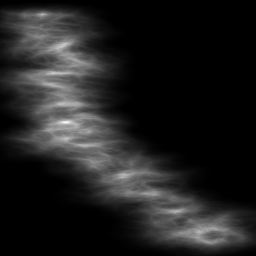
\includegraphics[width=0.49\textwidth]{Memoria/images/mountain_delta.png}
    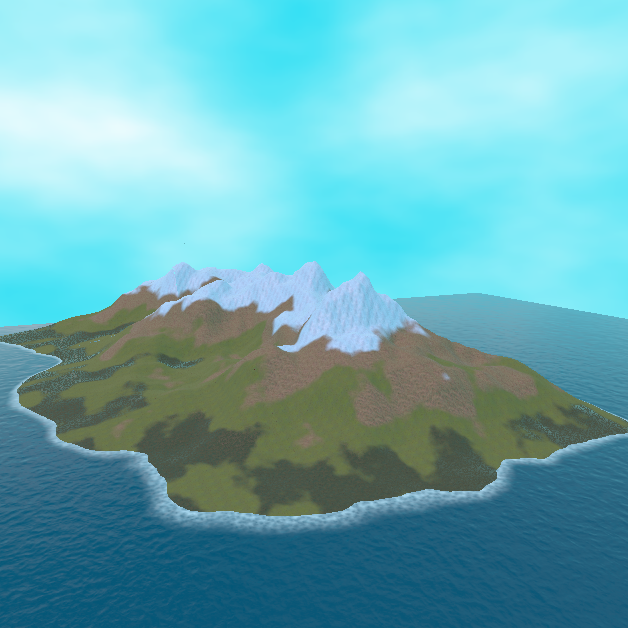
\includegraphics[width=0.49\textwidth]{Memoria/images/rendered_mountain_agent.png}
    \caption{Delta map generated by a \href{https://github.com/fsande/TFG---Eric-Rios/blob/main/Godot-TerrainGeneration/terrain_generation/agents/mountain_agent.gd}{\texttt{MountainAgent}} and its 3D representation.}
    \label{fig:mountain_delta}
\end{figure}
%% ===================================================


\subsection[\texttt{RiverAgent}]{\href{https://github.com/fsande/TFG---Eric-Rios/tree/main/Godot-TerrainGeneration/terrain_generation/agents/river}{\texttt{RiverAgent}}\footnote{\href{https://github.com/fsande/TFG---Eric-Rios/tree/main/Godot-TerrainGeneration/terrain_generation/agents/river}{\textit{Godot-TerrainGeneration/terrain\_generation/agents/river/river\_agent.gd}}}}

Also based on the pseudocode provided by \cite{Doran:2010:CPT}.
It randomly selects mountain and coast points and scores them, taking into account whether they are separated by sea as well as user-provided parameters.
A well-scored pair is chosen and a path between them is generated, following the terrain gradient up, starting at the coast and ending at the mountain (reverse water flow).
Then, a downward pass is done to ensure the path's validity and perform the carving (generating a delta map).

To expand upon the reference implementation this agent also makes use of the Feature Placement system (see Section \ref{sec:feature-placement}) to place a water mesh along the river's path.
This allows for rivers to exist not just at sea level and properly flow down from the mountains.
The gradient is encoded into the mesh's colour for shaders to use it for water flow direction.
An example of river generation is exhibited in Figure \ref{fig:river_agent}.

%% ===================================================
\begin{figure}[H]
    \centering
    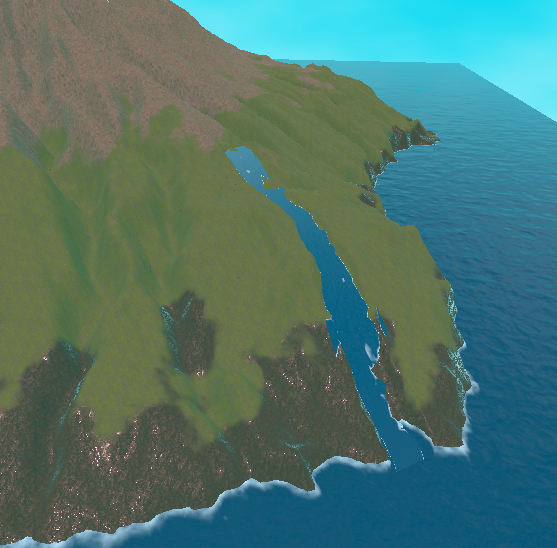
\includegraphics[width=0.5\textwidth]{Memoria/images/river_example.png}
    \caption{River agent applied on top of the heightmap displayed in Figure \ref{fig:texture_heightmap_source}. 
    It finds a pre-existing ravine, modifies it and places the water mesh.}
    \label{fig:river_agent}
\end{figure}
%% ===================================================

\subsection[\texttt{TunnelAgent}]{\href{https://github.com/fsande/TFG---Eric-Rios/blob/main/Godot-TerrainGeneration/terrain_generation/agents/tunnels/tunnel_boring_agent.gd}{\texttt{TunnelAgent}}\footnote{\href{https://github.com/fsande/TFG---Eric-Rios/blob/main/Godot-TerrainGeneration/terrain\_generation/agents/tunnels/tunnel\_boring\_agent.gd}{\textit{Godot-TerrainGeneration/terrain\_generation/agents/tunnels/tunnel\_boring\_agent.gd}}}}

The tunnel agent is the most ambitious of the implemented agents.
It has been created as a proof of concept for more complex cave generation systems, not typical in heightmap and mesh based terrain, but mostly seen on voxel systems.
The struggles in its implementation have illustrated why voxel systems are generally preferred for cave generation.
However, the \href{https://github.com/fsande/TFG---Eric-Rios/blob/main/Godot-TerrainGeneration/terrain_generation/agents/tunnels/tunnel_boring_agent.gd}{\texttt{TunnelAgent}} has been successful. 
It uses \href{https://github.com/fsande/TFG---Eric-Rios/blob/main/Godot-TerrainGeneration/terrain_generation/agents/volume_definition.gd}{\texttt{VolumeDefinition}} to carve an entrance to the tunnel and generates a configurable tunnel mesh, which is then added to the terrain.
A tunnel generated on a snowy cliff is displayed in Figure \ref{fig:tunnel_agent}

%% ===================================================
\begin{figure}[H]
    \centering
    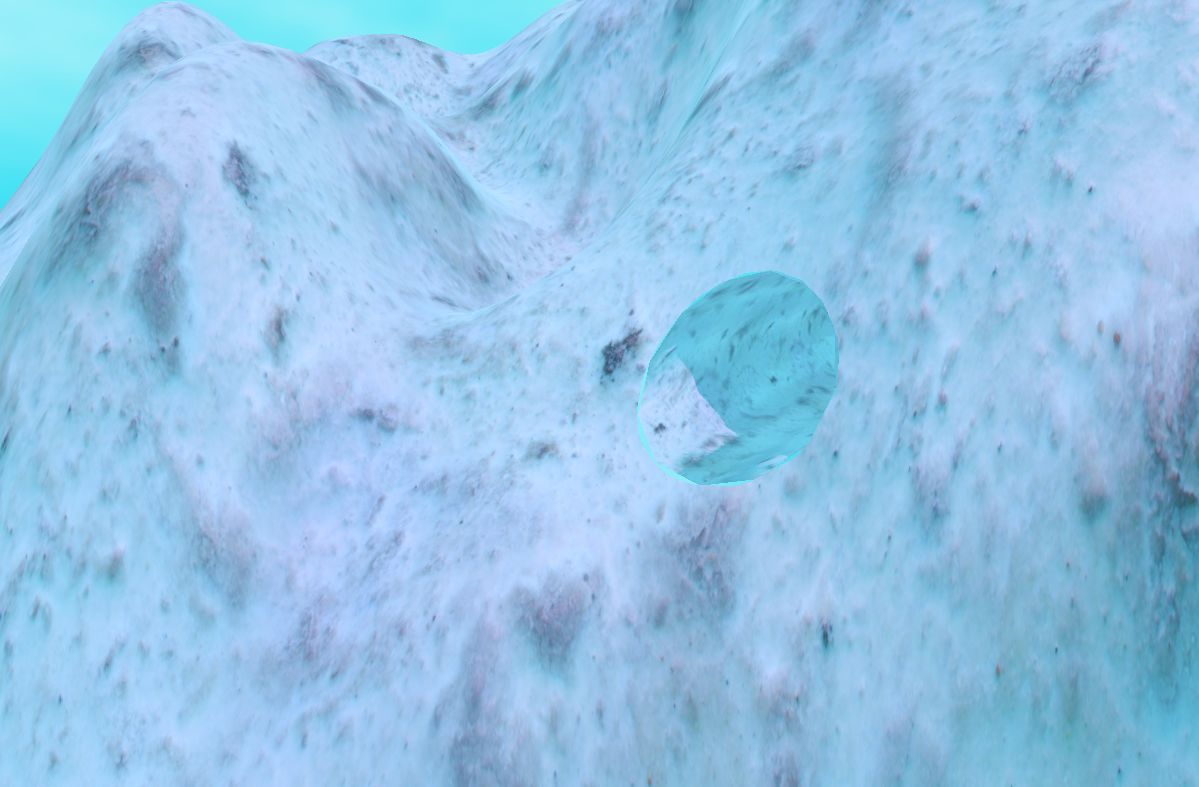
\includegraphics[width=0.75\textwidth]{Memoria/images/snowy_tunnel.png}
    \caption{Tunnel agent on \textit{Simplex} noise.}
    \label{fig:tunnel_agent}
\end{figure}
%% ===================================================

\subsection[\texttt{OverhangAgent}]{\href{https://github.com/fsande/TFG---Eric-Rios/blob/main/Godot-TerrainGeneration/terrain_generation/agents/overhang_agent.gd}{\texttt{OverhangAgent}}\footnote{\href{https://github.com/fsande/TFG---Eric-Rios/blob/main/Godot-TerrainGeneration/terrain_generation/agents/overhang_agent.gd}{\textit{Godot-TerrainGeneration/terrain\_generation/agents/overhang\_agent.gd}}}}

This is another agent that makes use of \href{https://github.com/fsande/TFG---Eric-Rios/blob/main/Godot-TerrainGeneration/terrain_generation/agents/volume_definition.gd}{\texttt{VolumeDefinition}}, allowing for volumetric modifications of the terrain.
It is designed to run after the initial height generation, identify points where an overhang could be added according to user parameters and generates meshes correspondingly.
This agent's current implementation works mainly as a prototype for the volume generation and cliff-finding algorithms, as the generated meshes are fairly low quality compared to those produced by the other implemented methods.
However, they could be suitable for a stylized ‘low-poly’ aesthetic.
Some generated overhangs can be appreciated in Figure \ref{fig:overhangs}.
%% ===================================================
\begin{figure}[H]
    \centering
    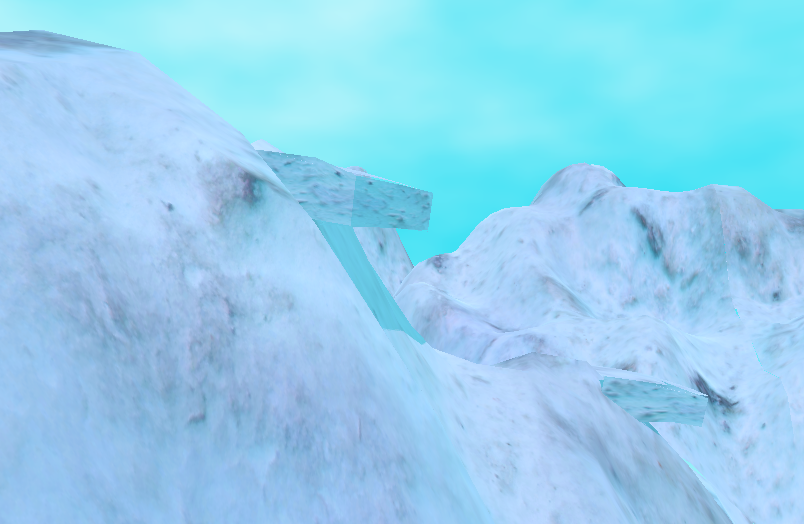
\includegraphics[width=0.75\textwidth]{Memoria/images/overhangs.png}
    \caption{Overhangs generated on \textit{Simplex} noise base.}
    \label{fig:overhangs}
\end{figure}
%% ===================================================
\section{Feature Placement}
\label{sec:feature-placement}

Up to this point the implementation has concerned itself with the terrain's geography.
Methods to generate mountains, valleys, rivers and caves have been explored.
Nevertheless, the terrain looks empty without other features, such as vegetation, sporadic rock formations and others.
The \href{https://github.com/fsande/TFG---Eric-Rios/blob/main/Godot-TerrainGeneration/terrain_generation/chunking/chunk_feature.gd}{\texttt{ChunkFeature}}\footnote{\href{https://github.com/fsande/TFG---Eric-Rios/blob/main/Godot-TerrainGeneration/terrain_generation/chunking/chunk_feature.gd}{\textit{Godot-TerrainGeneration/terrain\_generation/chunking/chunk\_feature.gd}}} system aims to solve this by providing a controllable and extensible way of adding custom assets to the scene in an organic manner that fits the rest of the workflow.
The user can define a list of \href{https://github.com/fsande/TFG---Eric-Rios/blob/main/Godot-TerrainGeneration/terrain_generation/props/prop_placement_rule.gd}{\texttt{PropPlacementRule}s}\footnote{\href{https://github.com/fsande/TFG---Eric-Rios/blob/main/Godot-TerrainGeneration/terrain_generation/props/prop_placement_rule.gd}{\textit{Godot-TerrainGeneration/terrain\_generation/props/prop\_placement\_rule.gd}}}, a subclass of \href{https://github.com/fsande/TFG---Eric-Rios/blob/main/Godot-TerrainGeneration/terrain_generation/chunking/chunk_feature.gd}{\texttt{ChunkFeature}}, just like the \href{https://github.com/fsande/TFG---Eric-Rios/blob/main/Godot-TerrainGeneration/terrain_generation/agents/river/river_water_feature.gd}{\texttt{RiverWaterFeature}}\footnote{\href{https://github.com/fsande/TFG---Eric-Rios/blob/main/Godot-TerrainGeneration/terrain_generation/agents/river/river_water_feature.gd}{\textit{Godot-TerrainGeneration/terrain\_generation/agents/river/river\_water\_feature.gd}}} used by \href{https://github.com/fsande/TFG---Eric-Rios/tree/main/Godot-TerrainGeneration/terrain_generation/agents/river}{\texttt{RiverAgent}}.
These rules take a \texttt{PackedScene}\footnote{\href{https://docs.godotengine.org/en/stable/classes/class_packedscene.html}{\texttt{PackedScene} Godot Documentation\\ \hspace*{1.9em}\url{https://docs.godotengine.org/en/stable/classes/class_packedscene.html}}}(the environmental asset (prop) to be instanced), a density and optional density map, as well as an array of \href{https://github.com/fsande/TFG---Eric-Rios/blob/main/Godot-TerrainGeneration/terrain_generation/props/constraints/prop_placement_constraint.gd}{\texttt{PropPlacementConstraint}s}\footnote{\href{https://github.com/fsande/TFG---Eric-Rios/blob/main/Godot-TerrainGeneration/terrain_generation/props/constraints/prop_placement_constraint.gd}{\textit{Godot-TerrainGeneration/terrain\_generation/props/constraints/prop\_placement\_constraint.gd}}}.
These are varied and make use of polymorphism to allow for extensibility.
As of this point in development, the following constraints have been implemented: 
\begin{itemize}
    \item \href{https://github.com/fsande/TFG---Eric-Rios/blob/main/Godot-TerrainGeneration/terrain_generation/props/constraints/height_range_constraint.gd}{\texttt{HeightRangeConstraint}}: Ensures that the props are only placed within a specified height range.
    \item \href{https://github.com/fsande/TFG---Eric-Rios/blob/main/Godot-TerrainGeneration/terrain_generation/props/constraints/sea_level_constraint.gd}{\texttt{SeaLevelConstraint}}: Specific case of \href{https://github.com/fsande/TFG---Eric-Rios/blob/main/Godot-TerrainGeneration/terrain_generation/props/constraints/height_range_constraint.gd}{\texttt{HeightRangeConstraint}} which automatically adapts to the configured sea level. 
    It can constrain props to always appear above or below sea.
    \item \href{https://github.com/fsande/TFG---Eric-Rios/blob/main/Godot-TerrainGeneration/terrain_generation/props/constraints/slope_range_constraint.gd}{\texttt{SlopeRangeConstraint}}: Ensures that props are only placed within a specified slope range.
    \item \href{https://github.com/fsande/TFG---Eric-Rios/blob/main/Godot-TerrainGeneration/terrain_generation/props/constraints/spacing_constraint.gd}{\texttt{SpacingConstraint}}: Ensures a minimum distance between props to avoid geometry clipping or too much density.
    \item \href{https://github.com/fsande/TFG---Eric-Rios/blob/main/Godot-TerrainGeneration/terrain_generation/props/constraints/volume_exclusion_constraint.gd}{\texttt{VolumeExclusionConstraint}}: Prevents props from being placed inside of subtracted volumes, such as tunnels.
    \item \href{https://github.com/fsande/TFG---Eric-Rios/blob/main/Godot-TerrainGeneration/terrain_generation/props/constraints/zone_constraint.gd}{\texttt{ZoneConstraint}}: \href{https://github.com/fsande/TFG---Eric-Rios/blob/main/Godot-TerrainGeneration/terrain_generation/core/height_delta_map.gd}{\texttt{HeightDeltaMap}}s can be tagged by agents with specific zone tags of the \texttt{StringName}\footnote{\href{https://docs.godotengine.org/en/stable/classes/class_stringname.html}{\texttt{StringName} Godot Documentation}\\ \hspace*{1.9em}\url{https://docs.godotengine.org/en/stable/classes/class_stringname.html}} type.
    Props will not spawn there.
\end{itemize}

Props can also make use of Godot's \texttt{MultiMesh}\footnote{\href{https://docs.godotengine.org/en/stable/classes/class_multimesh.html}{Godot Multimesh Documentation}\\ \hspace*{1.9em}\url{https://docs.godotengine.org/en/stable/classes/class_multimesh.html}} implementation to reduce GPU calls and their overhead.

The props will only be placed in LODs under a given threshold and their density will diminish as they get farther away in LOD.
This, coupled with the rest of optimizations, allows for performance-friendly dense prop instantiation, as seen in Figure \ref{fig:prop_placement}.

%% ===================================================
\begin{figure}[H]
    \centering
%    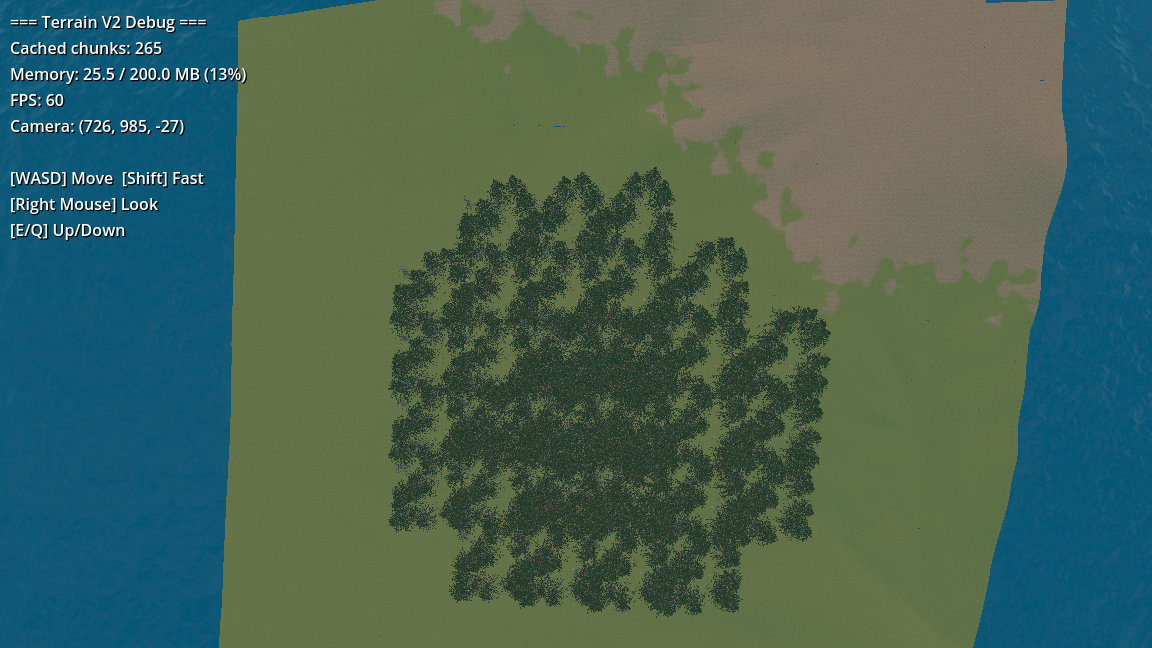
\includegraphics[width=1\textwidth]{Memoria/images/props_far_away.png}
    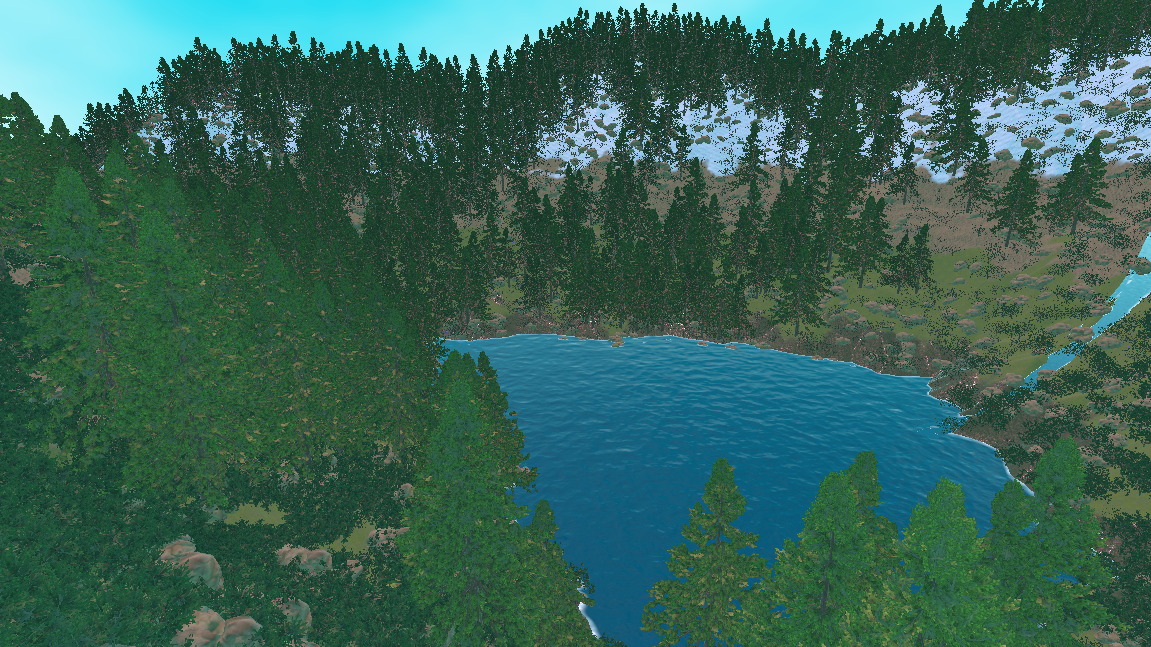
\includegraphics[width=1\textwidth]{Memoria/images/props_example.png}
    \caption{First person perspective of features (trees, bushes, rocks and a river), running at stable 60 FPS}
    \label{fig:prop_placement}
\end{figure}
%% ===================================================


\section{Chunking and Level of Detail}
\label{sec:chunking_and_lod}

Procedural terrain generation of large worlds runs into the problem of scale. 
It is desired for the terrain to be extensive, but it must also be of good visual quality, as well as performant.
This project has implemented DLOD \cite{Dalei:2022:RLB} through chunking to achieve this.

\subsection{Mesh Generation}
Each chunk has its own mesh and, as such, must be generated independently. Two methods have been implemented to generate chunk meshes: one for CPU and another for GPU.
Like much of the project they have been implemented following the Strategy pattern, providing a shared interface and allowing future extension with new strategies.
During development this proved useful when migrating from a GDScript CPU implementation to a C++ one, as it allowed for quick switching between strategies for benchmarking purposes.
Although the GPU method has proven to be more efficient for higher resolution chunks (see Chapter \ref{chap:Evaluation}), it does not allow for asynchronous generation, due to Godot's blocking access to most of \texttt{RenderingDevice}'s\footnote{\href{https://docs.godotengine.org/en/stable/classes/class_renderingdevice.html}{\texttt{RenderingDevice} Godot Documentation}\\ \hspace*{1.9em}\url{https://docs.godotengine.org/en/stable/classes/class_renderingdevice.html}} features from outside the main thread, completely nullifying the benefits provided by asynchronicity.
The \texttt{buffer\_get\_data\_async()} method can be used from the main thread, but bandwidth limitations and synchronization still make it inappropriate for real time generation.
This has made the CPU method a clear victor for the default option, as it can generate chunks on demand without blocking the main thread without causing frame drops during gameplay.

The CPU chunk generation has been implemented in C++ using GDExtension\footnote{\href{https://docs.godotengine.org/en/4.x/tutorials/scripting/gdextension/index.html}{GDExtension Documentation} - \url{https://tinyurl.com/gdextension}}.
It was originally prototyped in GDScript, like the rest of the project.
However, during benchmarking, it proved to be a bottleneck in gameplay.
After analysis, it was discovered that GDScript code does not utilize threads well and the interpreter performs many blocking operations.
Migrating chunk generation to C++ has shown around 34.68x faster performance sequentially and 81.80x in parallel, as will be more carefully illustrated in Chapter \ref{chap:Evaluation}.
% TODO: Información sobre implementación concreta de algoritmos si queda espacio

\subsection{Level of Detail}
The number of LODs can be defined by the user, starting at 0, the highest quality and generating chunks of \texttt{base\_chunk\_resolution} subdivisions.
As the LOD increases, the number of subdivisions gets halved (e.g. for \texttt{base\_chunk\_resolution = 64} a chunk on LOD 2 would have 16 subdivisions).
This is achieved by halving the sampling rate on the heightmap.
An example of different LODs for a same chunk can be seen in Figure \ref{fig:lod_levels}.

%% ===================================================
\begin{figure}[H]
    \centering
    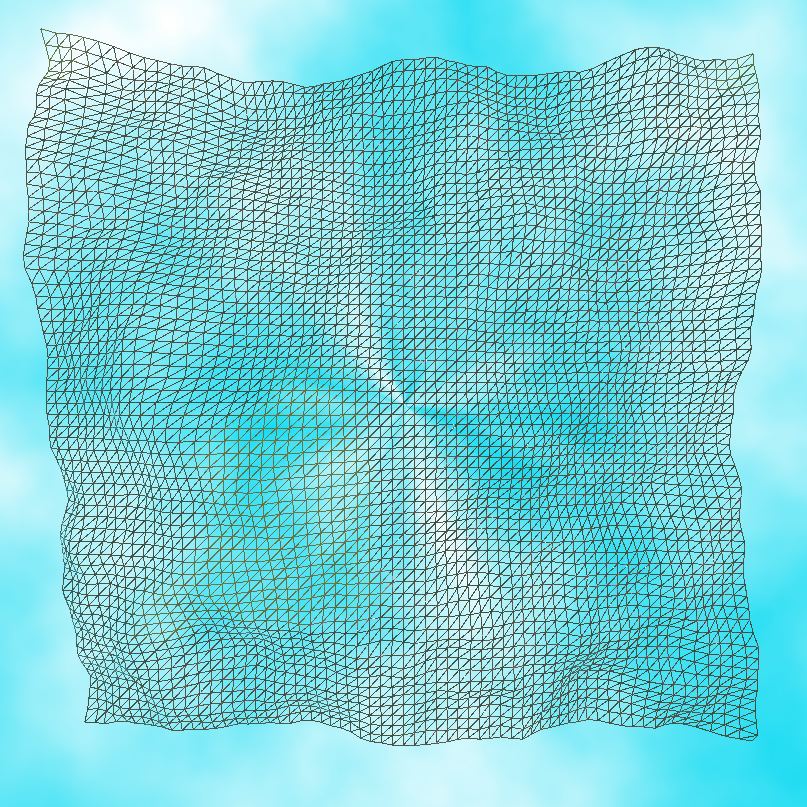
\includegraphics[width=0.48\textwidth]{Memoria/images/lod0.png}
    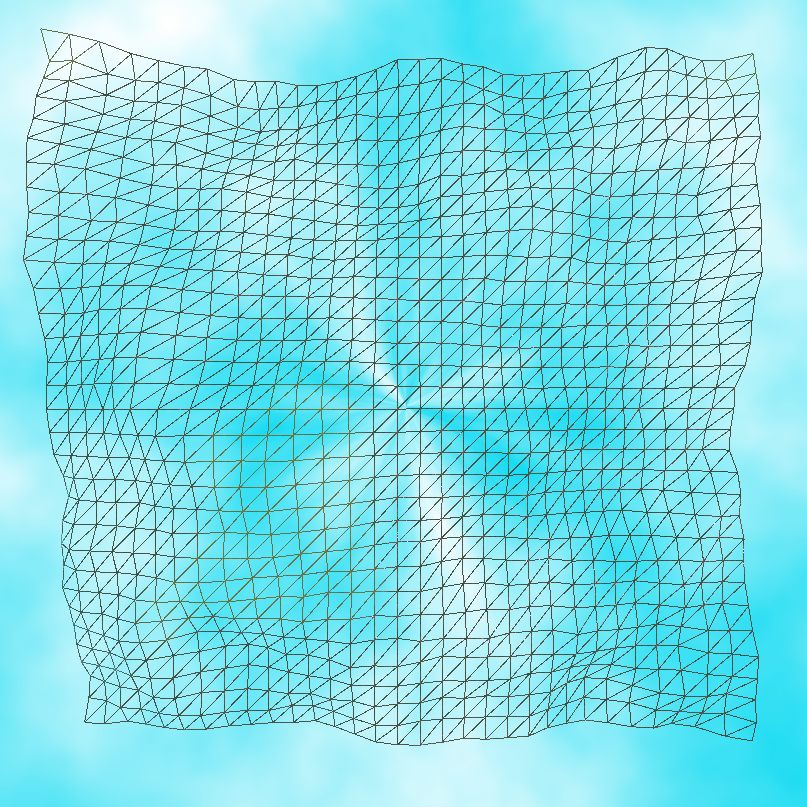
\includegraphics[width=0.48\textwidth]{Memoria/images/lod1.png}
    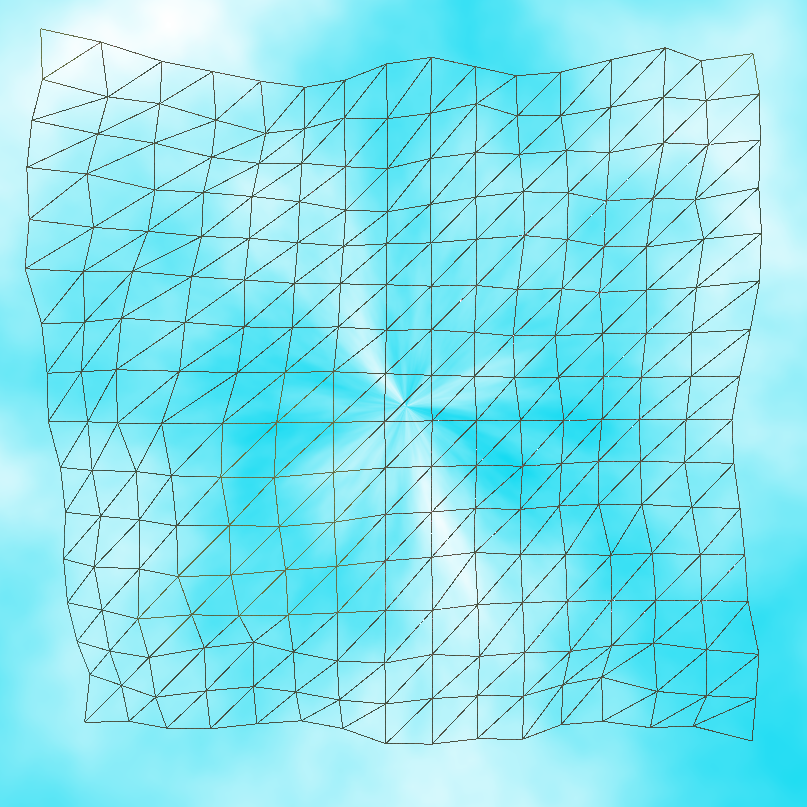
\includegraphics[width=0.48\textwidth]{Memoria/images/lod2.png}
    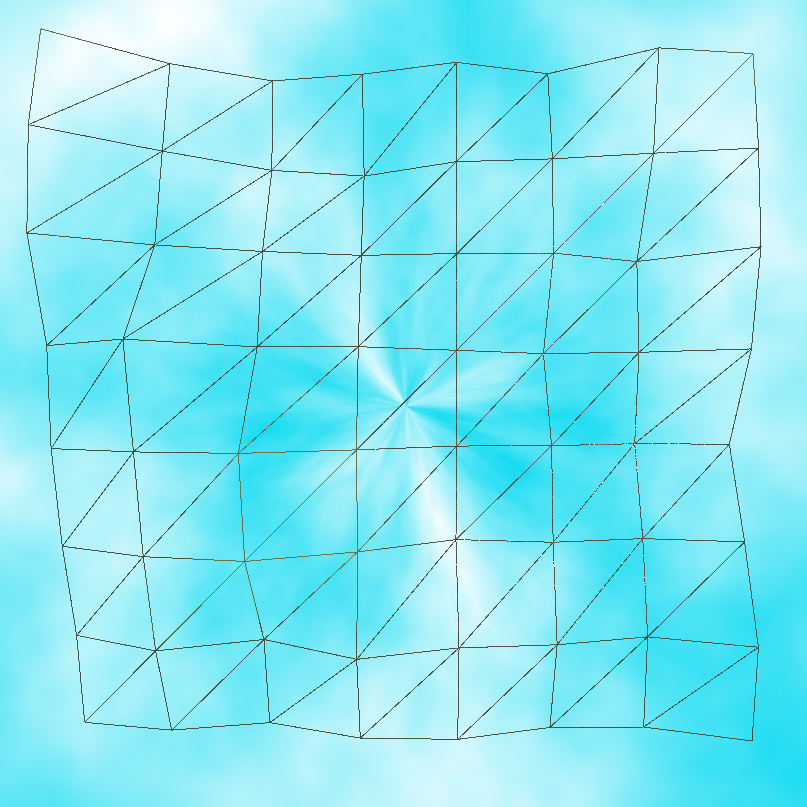
\includegraphics[width=0.48\textwidth]{Memoria/images/lod3.png}
    \caption{A chunk in LOD levels 0 to 3. (With \texttt{base\_chunk\_resolution} = 64).}
    \label{fig:lod_levels}
\end{figure}
%% ===================================================

\subsection{Asynchronicity}
To allow for continuous gameplay without freezing, it is crucial for the chunking system to be asynchronous.
To achieve an extensible and configurable async chunk generation and loading system, three main strategies have been applied.
\begin{enumerate}
    \item \textbf{Chunk caching} - 
        Chunks are cached in an LRU cache implemented using a \texttt{Dictionary} with the chunk's coordinates as keys.
        The cache's size is user-defined.
    \item \textbf{Request queue with priorities} - A \href{https://github.com/fsande/TFG---Eric-Rios/blob/main/Godot-TerrainGeneration/terrain_generation/chunking/chunk_request_queue.gd}{\texttt{ChunkRequestQueue}}\footnote{\href{https://github.com/fsande/TFG---Eric-Rios/blob/main/Godot-TerrainGeneration/terrain_generation/chunking/chunk_request_queue.gd}{\textit{Godot-TerrainGeneration/terrain\_generation/chunking/chunk\_request\_queue.gd}}} has been implemented that takes \href{https://github.com/fsande/TFG---Eric-Rios/blob/main/Godot-TerrainGeneration/terrain_generation/chunking/chunk_request.gd}{\texttt{ChunkRequest}s}\footnote{\href{https://github.com/fsande/TFG---Eric-Rios/blob/main/Godot-TerrainGeneration/terrain_generation/chunking/chunk_request.gd}{\textit{Godot-TerrainGeneration/terrain\_generation/chunking/chunk\_request.gd}}} and manages their generation.
    It makes use of Godot's \texttt{Thread}s\footnote{\href{https://docs.godotengine.org/en/stable/classes/class_thread.html}{\texttt{Thread} Godot Documentation}} to provide asynchronous generation.
    \item \textbf{Frame budgeting at instantiation} - The user can define what percentage of a frame's time chunk instantiation should take at most.
    Each time a chunk is requested, the system heuristically checks whether the remaining budget is enough. 
    If it is not, the instantiation is postponed to the next frame.
    In this way the frame-rate is kept stable.
\end{enumerate}

\subsection{Load Strategies}
Different \href{https://github.com/fsande/TFG---Eric-Rios/blob/main/Godot-TerrainGeneration/terrain_generation/chunking/strategies/chunk_load_strategy.gd}{\texttt{ChunkLoadStrategy}}\footnote{\href{https://github.com/fsande/TFG---Eric-Rios/blob/main/Godot-TerrainGeneration/terrain_generation/chunking/strategies/chunk_load_strategy.gd}{\textit{Godot-TerrainGeneration/terrain\_generation/chunking/strategies/chunk\_load\_strategy.gd}}} implementations have been developed to decide which chunks at which LOD and priority are loaded and unloaded.
A visualization of the implemented strategies can be seen in Figure \ref{fig:generation_strategies}.

\begin{itemize}
    \item \href{https://github.com/fsande/TFG---Eric-Rios/blob/main/Godot-TerrainGeneration/terrain_generation/chunking/strategies/grid_load_strategy.gd}{\texttt{GridLoadStrategy}}: Chunks below a given radius around the camera are loaded and those outside of another defined radius are unloaded.
    \item \href{https://github.com/fsande/TFG---Eric-Rios/blob/main/Godot-TerrainGeneration/terrain_generation/chunking/strategies/view_load_strategy.gd}{\texttt{ViewLoadStrategy}}: Chunks in a radius around the camera with a given angle from its forward vector are loaded and those outside of that zone are unloaded.
    \item \href{https://github.com/fsande/TFG---Eric-Rios/blob/main/Godot-TerrainGeneration/terrain_generation/chunking/strategies/grid_and_view_load_strategy.gd}{\texttt{GridAndViewLoadStrategy}}: Combines both previous strategies. 
    A chunk is loaded if either strategy requests it, and unloaded only if both agree it should be.
\end{itemize}

%% ===================================================
\begin{figure}[H]
    \centering
    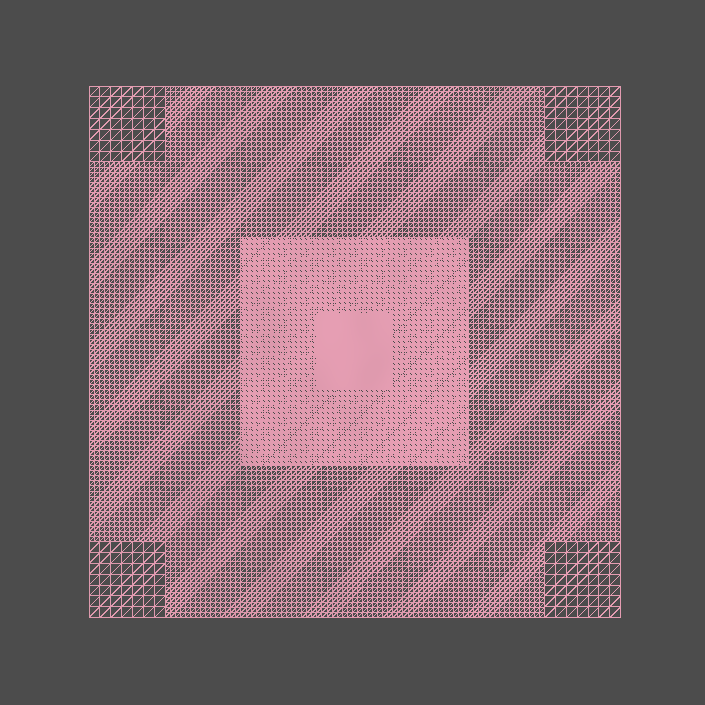
\includegraphics[width=0.32\textwidth]{Memoria/images/grid_load_chunks.png}
    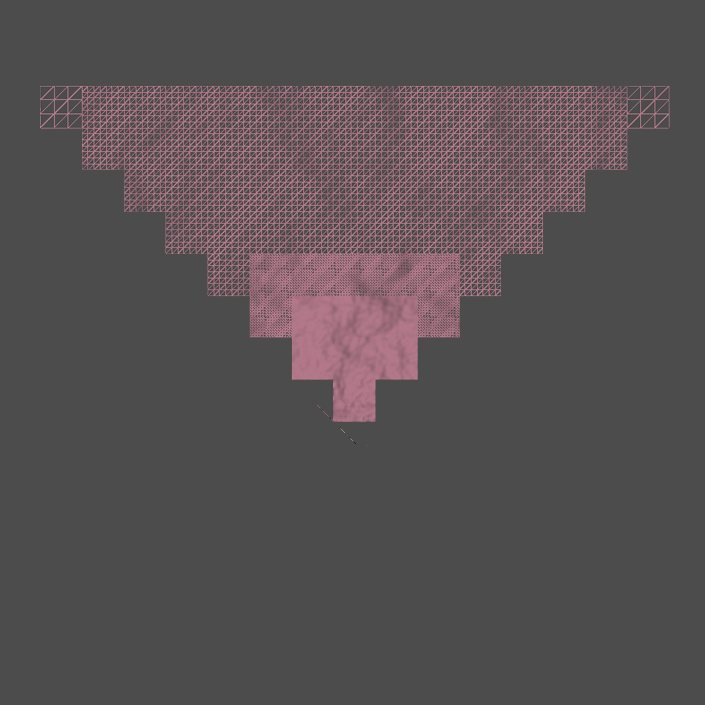
\includegraphics[width=0.32\textwidth]{Memoria/images/view_load_chunks.png}
    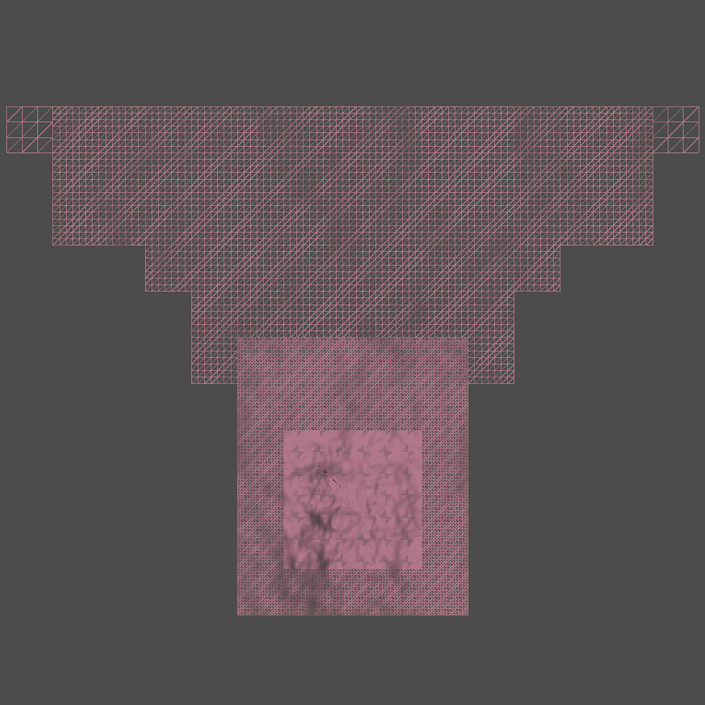
\includegraphics[width=0.32\textwidth]{Memoria/images/grid_and_view_load_chunks.png}
    \caption{From left to right: Chunks loaded with \href{https://github.com/fsande/TFG---Eric-Rios/blob/main/Godot-TerrainGeneration/terrain_generation/chunking/strategies/grid_load_strategy.gd}{\texttt{GridLoadStrategy}}, \href{https://github.com/fsande/TFG---Eric-Rios/blob/main/Godot-TerrainGeneration/terrain_generation/chunking/strategies/view_load_strategy.gd}{\texttt{ViewLoadStrategy}} and \href{https://github.com/fsande/TFG---Eric-Rios/blob/main/Godot-TerrainGeneration/terrain_generation/chunking/strategies/grid_and_view_load_strategy.gd}{\texttt{GridAndViewLoadStrategy}}. 
    The decreasing density can be appreciated as chunks get farther away.}
    \label{fig:generation_strategies}
\end{figure}
%% ===================================================

\section{Collision Generation}

Collision in a video game is the detection of objects touching or overlapping. 
The generated terrain needs collision if a player is expected to traverse it, otherwise they would fall through.
The collision is generated on a per-chunk basis and uses the chunk's mesh as a basis, using the \texttt{create\_trimesh\_shape()} method, which generates a \texttt{ConcavePolygonShape3D}\footnote{\href{https://docs.godotengine.org/en/latest/classes/class_concavepolygonshape3d.html}{\texttt{ConcavePolygonShape3D} Documentation}\\ \hspace*{1.9em}\url{https://docs.godotengine.org/en/4.x/classes/class_concavepolygonshape3d.html}}.

Collision generation and instantiation are fairly computationally expensive and need to happen invisibly at runtime.
Several methods have been implemented to make the process as performant as possible.
The collision shape for each chunk is generated on a separate thread, making it non-blocking. 
The instantiation must happen in the main thread, but is fast enough not to be apparent when densities are not too high.
Collision is only generated for chunks that are located in a user-defined radius around the player.
This ensures that terrain close to the player can be collided with, without generating collision for faraway geometry not in current reach.
Since lower-fidelity collision is not significantly noticeable compared to the visual geometry, particularly during traversal, the mesh LOD system can also be used to generate simplified collision meshes, as displayed in Figure \ref{fig:collision_lod}.
The user can specify which LOD they want the generated collisions to have relative to the visual one.
This makes it so generation and instantiation are faster and reduces computation during gameplay.

%% ===================================================
\begin{figure}[H]
    \centering
    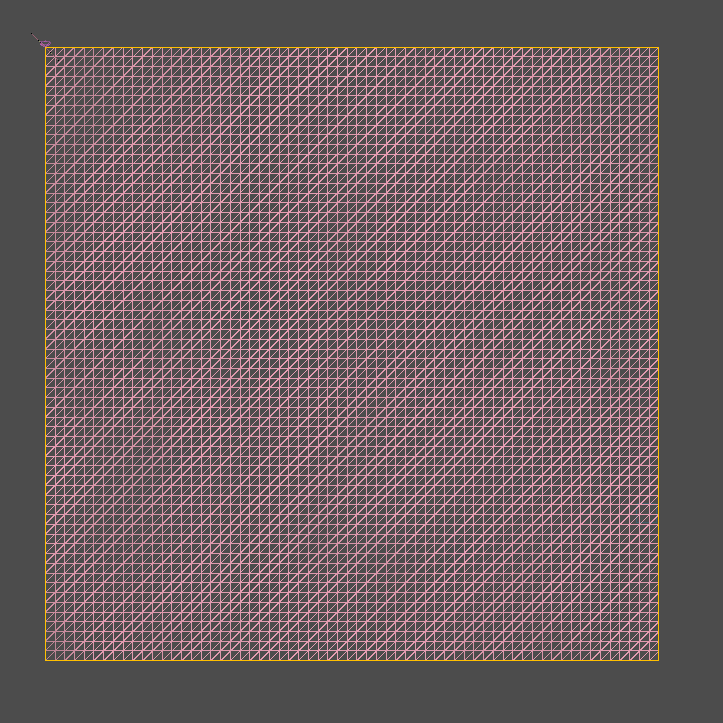
\includegraphics[width=0.49\textwidth]{Memoria/images/mesh_lod_0.png}
    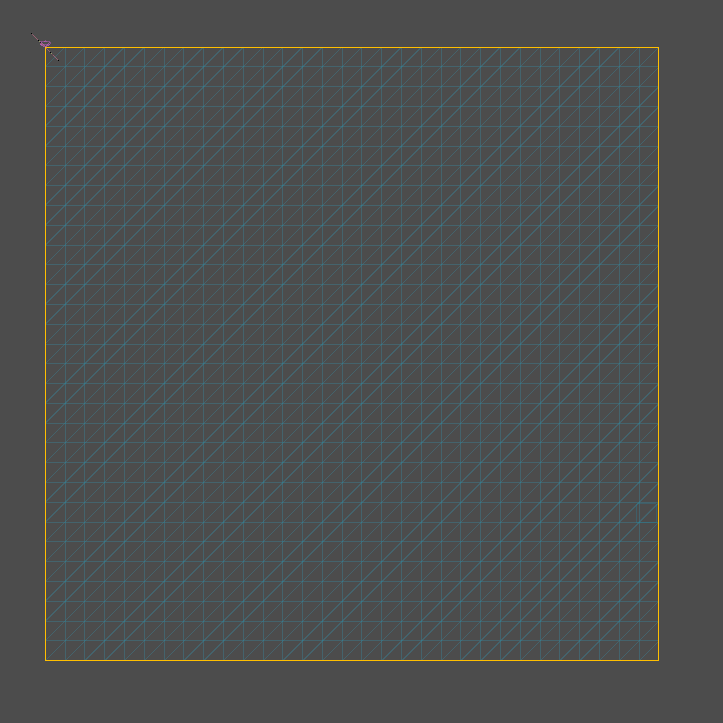
\includegraphics[width=0.49\textwidth]{Memoria/images/mesh_col.png}
    \caption{A chunk with visual LOD 0 (left), but collision LOD1 (right)).}
    \label{fig:collision_lod}
\end{figure}
%% ===================================================
